\DocumentMetadata{lang=en-US}

\documentclass[12pt,oneside,letterpaper]{report}


\usepackage{amsmath}

\usepackage[T1]{fontenc}
\usepackage{txfonts}
\usepackage{microtype}

\usepackage{graphicx}	% Including figure files
\usepackage{booktabs}
\usepackage{longtable}
\graphicspath{{../figures/}} 
\usepackage{isotope}
\usepackage[tableposition=above]{caption}

\usepackage{aas_macros}
\usepackage{natbib}
\usepackage[nottoc,numbib]{tocbibind}
\setcitestyle{aysep={}} 
\setcitestyle{notesep={; }} 


\usepackage{hyperref}
\hypersetup{
    colorlinks=true,
    linkcolor=black,
    filecolor=black,
    urlcolor=black,
    citecolor=black,
    pdftitle={The Galactic Chemical Evolution of Carbon},
    pdfauthor={Daniel A Boyea},
    pdfcreator={Themself},
    pdfkeywords={astronomy, supernovae, modeling, stellar yields, chemical evolution, galaxies, carbon},
}

\urlstyle{same}


%%%%%%%%%%%%%%% Formatting %%%%%%%%%%%%%%%%%%
\usepackage{titlesec}

\titleformat{\chapter}{\normalfont\normalsize\centering\bf}{\thechapter.}{1em}{}
\titleformat{\section}{\normalfont\normalsize\centering}{\thesection}{1em}{}
\titleformat{\subsection}{\normalfont\normalsize\centering}{\thesubsection}{1em}{}
% \titlespacing*{\chapter}{0pt}{0pt}{40pt} 
% \titlespacing*{\section}{0pt}{0pt}{20pt}
\renewcommand{\contentsname}{Table of Contents}
\AtBeginDocument{
      \renewcommand{\bibsection}{\chapter*{\bibname}}
  }


\usepackage{etoolbox}% http://ctan.org/pkg/etoolbox
\makeatletter
% \patchcmd{<cmd>}{<search>}{<replace>}{<succes>}{<failure>}
\patchcmd{\@chapter}{\addtocontents{lof}{\protect\addvspace{10\p@}}}{}{}{}% LoF
\patchcmd{\@chapter}{\addtocontents{lot}{\protect\addvspace{10\p@}}}{}{}{}% LoT
\makeatother

\pagestyle{plain}
\counterwithout{figure}{chapter}
\counterwithout{table}{chapter}
\counterwithout{equation}{chapter}

\newcommand\T{\rule{0pt}{2.6ex}}       % Top strut
\newcommand\B{\rule[-1.2ex]{0pt}{0pt}} % Bottom strut



\usepackage{accsupp}
\usepackage[accsupp]{axessibility}

%%%%%%%%%%%%%%% Acronyms %%%%%%%%%%%%%%%%%%
\usepackage[acronym,automake,symbols,
nogroupskip,
accsupp,
counter=section,
stylemods={longextra}
]{glossaries-extra}
\makeglossaries

\setabbreviationstyle[acronym]{long-short-sc}
\GlsXtrEnablePreLocationTag{\S }{\S }


\newacronym
[ description ={Core collapse supernovae. Massive star explosions. {\sc Ccsne} produce many elements including \gls{alpha}, \gls{fepeak}, and r and \gls{sproc}.}
]
{cc}{ccsne}{core collapse supernovae}

\newacronym
[description={Asymptotic giant branch stars. The {\sc agb} phase is the last phase of \glspl{lowmass}, before stars become white dwarfs. Produces C, N, and heavy \gls{sproc} elements. See \ref{sec:stel_evo}.}.]
{agb}{agb}{asymptotic giant branch}

\newacronym
[description={Type Ia Supernovae. Exploding white dwarfs. Produces \gls{fepeak} and has a long delay time.}]
{ia}{sne ia}{supernovae type Ia}


\newacronym
[description={Galactic chemical evolution.}]
{gce}{gce}{galactic chemical evolution}

\newacronym
[description={Star formation history.}]
{sfh}{sfh}{star formation history}

\newacronym
[description={Single stellar population. A group of stars formed all at the same time.}]
{ssp}{ssp}{single stellar population}

\newacronym
[description={Initial mass function. A function describing the mass distribution of newly formed stars. I use a \citet{kroupa01} {\sc imf}, which is described as a piecewise power-law function of $M$.}]
{imf}{imf}{initial mass function}

\newacronym
[description={
Apache Point Observatory Galactic Evolution Experiment. 
A large near-infrared spectroscopic survey of stars in the Milky Way. \citep{apogee17}.}]
{apogee}{apogee}{Apache Point Observatory Galactic Evolution Experiment}

\newacronym
[
description={Damped Lyman-alpha system. {\sc dla}s are clouds of gas from the 
early universe which are observed through their absorption of quasar spectra. The name 
comes from the strong Lyman-alpha lines ($1216\AA$) due to H absorption.}
]
{dla}{dla}{damped Lyman-alpha systems}





\newcommand{\cc}{\gls{cc}}
\newcommand{\Cc}{\Gls{cc}}
\newcommand{\agb}{\gls{agb}}
\newcommand{\ia}{\gls{ia}}
\newcommand{\sfh}{\gls{sfh}}
\newcommand{\dla}{\gls{dla}}
\newcommand{\ssp}{\gls{ssp}}
\newcommand{\imf}{\gls{imf}}
\newcommand{\gce}{\gls{gce}}
\newcommand{\Gce}{\Gls{gce}}
\newcommand{\apogee}{\gls{apogee}}




%%%%%%%%%%%%%%%%%%%%%% terms %%%%%%%%%%%%%%%
\newglossaryentry{metallicity}{name={metallicity},
    description={the (mass) fraction of a star or gas which is not made of either H or He. For the sun, the metallicity is $\Zo = 0.014$}
}

\newglossaryentry{yield}{name={yield},
    description={The net production of a new element during a star's lifecycle divided by the star's mass (including winds and supernovae ejecta). }
}

\newglossaryentry{nucleosynthesis}{name={nucleosynthesis},
    description={The synthesis of new elements through fusion inside stars. See section \ref{sec:stel_evo}.}
}

\newglossaryentry{multizone}{name={multi-zone},
    description={A chemical evolution model where a galaxy is divided into several zones, each with different stars, gas, and properties. }
}

\newglossaryentry{onezone}{name={one-zone},
    description={A chemical evolution model where the gas is all the same composition, i.e. neglecting spatial variations.}
}

\newglossaryentry{alpha}{name={$\alpha$-element},
    description={Elements which are made up of $\alpha$-particles (He nuclei) throuch the triple-$\alpha$ process (see Eq.~\ref{eq:triple_alpha}). Essentially light, even-numbered elements like O, Mg, and Na.}
}

\newglossaryentry{fepeak}{name={Fe-peak elements},
    description={Fe and nearby elements, produced in \gls{cc} and \gls{ia}.}
}

\newglossaryentry{sproc}{name={s-process elements},
    description={Elements produced through slow neutron captures, typically in \agb\ stars.}
}

\newglossaryentry{rgb}{name={red giant branch},
    description={Red giant branch stars are stars that have completed hydrogen core burning and have expanded in size. See Appendix \ref{sec:stel_evo}.}
}

\newglossaryentry{tdu}{name={third dredge up},
    description={Third dredge up occurs inside \gls{agb} stars. During each thermal pulse, material is {\it dredged up} from the core, changing the chemical abundances of the stellar atmosphere. (While nominally called {\it third dredge up}, there are typically several third dredge ups.). See Appendix \ref{sec:stel_evo}.}
}

\newglossaryentry{fdu}{name={first dredge up},
    description={First dredge up occurs when a \gls{lowmass} enters the \gls{rgb} phase. Material from the core is brought to the surface, increasing N and decreasing C abundances. See Appendix \ref{sec:stel_evo}.}
}

\newglossaryentry{hbb}{name={hot bottom burning},
    description={Hot bottom burning occurs inside \agb\ stars. The base of the convective envelope becomes hot enough for CNO burning to initiate.}
}

\newglossaryentry{subgiant}{name={subgiant},
    description={A star in the process of leaving the main sequence and becoming a \gls{rgb}.}
}

\newglossaryentry{imfave}{name={\gls{imf}-averaged},
    description={Averaged over the initial-mass function ({\sc imf}). The {\imf}-weighted yield is the mass of the newly produced element divided by the mass of star formation for a single stellar population (see \ssp).}
}


\newglossaryentry{dtd}{name={delay time distribution},
    description={The distribution in time of when an element is produced 
    after a star formation event.}
}

\newglossaryentry{massloading}{name={mass loading},
    description={The strength of outflows relative to star formation. See also $\eta$. }
}

\newglossaryentry{lowalpha}{name={low-$\alpha$},
    description={The low-$\alpha$ sequence, as described by Eq.~\ref{eq:high_alpha}. }
}

\newglossaryentry{highalpha}{name={high-$\alpha$},
    description={The high-$\alpha$ sequence, as described by Eq.~\ref{eq:high_alpha}. }
}


\newglossaryentry{lowmass}{name={low-mass star},
    description={Stars with masses $\lesssim 8\,M_\odot$ which end life as a white dwarf. }
}

\newglossaryentry{highmass}{name={high-mass star},
    description={Stars with masses $\lesssim 8\,M_\odot$, which end as a neutron star, black hole, or supernovae.}
}

\newglossaryentry{insideout}{name={{\it insideout}},
    description={Our fiducial star formation history. The rate of star formation is highest towards the center of the galaxy and at earlier times. See Eq.~\ref{eq:inside_out}.}
}

\newglossaryentry{cno}{name={CNO cycle},
    description = { A proton-fusion cycle which occurs in \gls{rgb} stars 
        consisting of a chain of proton captures releasing a He nucleus ($\alpha$-particle) and energy. See Eq.~\ref{eq:cno_cycle}.
}
}





\defcitealias{james+21}{J21}
\newcommand{\citetjack}{Roberts et al.~(2023, in prep.)}
\newcommand{\citepjack}{(Roberts et al.~2023, in prep.)}
\newcommand{\citealtjack}{Robert et al.~2023, in prep.}

\newcommand{\cxi}{\texttt{\hyperlink{C11}{C11}}}
\newcommand{\kx}{\texttt{\hyperlink{K10}{K10}}}
\newcommand{\kxvi}{\texttt{\hyperlink{K16}{K16}}}
\newcommand{\vxiii}{\texttt{\hyperlink{V13}{V13}}}

\newcommand{\JJ}{\citetalias{james+21}}
\newcommand{\VICE}{\texttt{VICE}}
\newcommand{\caah}{[C/Mg]-[Mg/H]}
\newcommand{\caafe}{[C/Mg]-[Mg/Fe]}

\newcommand{\alp}{$\alpha$}

\newcommand{\Ycc}{\ensuremath{y_{\rm C}^{\rm CC}}}
\newcommand{\Yoc}{\ensuremath{y_{\rm Mg}^{\rm CC}}}
\newcommand{\Ycagb}{\ensuremath{y_{\rm C}^{\rm AGB}}}
\newcommand{\sun}{\odot}
\newcommand{\Z}{Z}
\newcommand{\Zo}{Z_{\sun}}

\newcommand{\proton}{\isotope[1][1]{p}}

\newcommand{\zoo}{\ensuremath{Z/Z_{\sun }}}
\newcommand{\Yct}{\ensuremath{y_{\rm C}}}



\newcommand{\about}[1]{${\sim} #1$}


\title{The Galactic Chemical Evolution of Carbon}
\author{Daniel A. Boyea}

\date{\today}


















\begin{document}
% \linespread{1.25}

\pagenumbering{roman}

\begin{titlepage}
   \begin{center}
       \textbf{The Galactic Chemical Evolution of Carbon}\\
       Implications for Stellar Nucleosynthesis\\
       \vspace*{3\baselineskip}
        Undergraduate Research Thesis\\
       \vspace*{3\baselineskip}
    Presented in partial fulfillment of the requirements for graduation \textit{with research distinction in Astronomy and Astrophysics} in the College of Arts and Sciences of The Ohio State University\\
       \vspace*{3\baselineskip}
        by\\
       \vspace*{3\baselineskip}
       {Daniel Alexander Boyea}\\
       \vspace*{3\baselineskip}
       The Ohio State University\\
       April 2023\\
       \vspace*{3\baselineskip}
       Project Advisors\\
       James W. Johnson, Department of Astronomy \\
       Professor David H. Weinberg, Department of Astronomy 
       \vfill
   \end{center}
\end{titlepage}



% Abstract of the paper
\chapter*{Abstract}
\addcontentsline{toc}{chapter}{Abstract}
% context
Limited knowledge of stellar physics leads to uncertainties in elemental yield predictions.
% aims
As an independent approach, I constrain the nucleosynthetic yields of C using multizone Galactic chemical evolution models.
% results
By matching the median trends of \caah\ and \caafe\ in  {\sc APOGEE} subgiant stars, I find that high-mass and low-mass stars contribute \about{80\%} and \about{20\%} of total C production respectively.
% 
To match the normalization of the trends, I estimate the massive star C/Mg yield ratio $\Ycc/\Yoc = 1.57 + 0.59 \left(Z/Z_\odot\right)$,  explaining the \caah\ trend when including the low mass C contribution.
%
Variations in the star formation history only slightly impact the low [Mg/Fe] tail of the [C/Mg]-[Mg/Fe] relation. However, most of the scatter in the \caah\ distribution can be attributed to measurement errors and radial migration. 
% 
Due to the degeneracy between the normalization of elemental yields and the strength of mass-loading in Galactic outflows, I am only able to constrain the relative yields of C/Mg and its metallicity dependence. While measurements of gas-phase C abundances are challenging, my model is broadly consistent with the [C/O]-[O/H] trend observed in compiled literature measurements.





\chapter*{Acknowledgements}
\addcontentsline{toc}{chapter}{Acknowledgements}


I hope that the people who helped me complete this project will appreciate how much they have helped me. This year has been an incredibly challenging journey---and perhaps I am not open enough about what it has been like. I undoubtedly would not have reached this day without everyone's help.

James Johnson---your mentorship and guidance throughout this project was critical. 
You helped me learn an incredible amount about being an astronomer, and I am forever grateful for how you have guided this project, through late nights and last-minute comments.  Wayne, for everything you do for everyone---you are the glue holding together our department and nobody can say thank you enough. 
David and Jennifer for helping this project move forward, by providing guidance at critical junctions and being part of my committee. Rolando, for being the non-astronomer thrown into this work, and pointing out the flaw of incomprehensibility in this work.

Even though you may have not been able to help me with the science, dear friends and family, you have been no less important in the completion of this work. 
Eric, even across the country, you have always been a point of support and stability, and I am always happy to be around you. Anya, you are a wonderful friend and I cannot thank you enough for your unconditional support this year, 
All my friends who are just wonderful, inspiring, and incredible people---Kaia, Maria, Autumn, Simon, Bailee, Aaliyah, Sanskruti, Alyssa, Harrison, Denis, Keith, and so many others. 
And my family (including Arya, my most lovable doodle)---I can not even being to thank you enough for simply helping me recover my health and make it to graduation. 








%% Lists

\tableofcontents
\listoffigures
\listoftables
\newpage
\pagenumbering{arabic}







%%%%%%%%%%%%%%%%%%%%%%%%%%%%%%%%%%%%%%%%%%%%%%%%%%

%%%%%%%%%%%%%%%%% BODY OF PAPER %%%%%%%%%%%%%%%%%%

\chapter{Introduction}

\Gce{} aims to understand the chemical enrichment and star formation histories of galaxies. At the core of \gce{} models are stellar \gls{yield}---the amount of each chemical element stars produce (or destroy). Each element is produced in different amounts by different stars, leaving traces of the Galaxy's evolutionary history. Through \textit{Galactic Archeology}, we can reconstruct the history of our galaxy by investigating clues left behind in stars.

Here, I aim to understand C enrichment---where it is produced and how its abundances evolve. C is unique nucleosynthetically, one of few light elements (along with N) produced in \agb{} stars \citep[e.g.][]{jennifer19, KL14}. C and N are well-studied elements since they are easy to observe in stellar spectra, even at the lowest metallicities \cite[e.g.][]{fabbian+09, nissen+14, lambert81, laird85, lambert86}. Additionally, C and N are used as age indicators in \gls{rgb} stars \citep{martig16, MG15, hasselquist19, vincenzo+21}.

Gas-phase [C/O] ratios%
%
\footnote{In this paper, I use the standard notation for chemical abundances. $[A/B] = \log_{10}\left(A/B\right) - \log_{10}\left(A_{\sun}/B_{\sun}\right)$, i.e. $[A/B]$ is the logarithm of the ratio between A and B, scaled such that $[A/B]=0$ for the sun. Solar abundances are as measured in \citet{asplund+09}.}%
%
---observed in very low \gls{metallicity}
\footnote{Astronomers are not chemists. By metallicity, I mean the (mass) fraction of any element which is not H or He, denoted by $Z$. For the sun, $Z_\odot=0.014$. }
, high redshift
\footnote{i.e. observed in the early universe.}
\dla{}---decrease with increasing [O/H] \citep{FN15, cooke+17}. Then, [C/O] increases above $\rm [O/H] \approx -1$ (\citealt{berg+19}; see discussion in section \ref{sec:gas}).
While we know C is produced in \agb{} stars and \cc{}, we still have a limited understanding of the magnitude and metallicity-dependence of each process.


Nucleosynthetic yields predicted by stellar evolution models are rife with uncertainties, despite their central role in \gce{} models, nucleosynthetic yields predicted by stellar evolution models are rife with uncertainties. The production rates of elements in stars are shaped by poorly understood processes, including mass loss, opacity, nuclear reaction rates, rotational mixing, convection, and explodability \citep{KL14,ventura+13, LC18, emily+21}.

\Gce{} models typically use unmodified nucleosynthetic predictions and attempt to create models matching observations by varying the \sfh{} and other evolutionary parameters. Here, I introduce C yields as an additional free parameter, determining which yield prescriptions reproduce Galactic abundance trends.
\cite{james+23} examined similar \gce{} models of N, an element whose production is closely related to C. They  found that trends in N and O abundances can be explained by the \gls{metallicity} dependence of relative N and O yields. Here, I extend their models to C, deriving similar constraints on C/Mg yields. I assess which yield prescriptions reproduce Galactic abundance trends while investigating the impact of \gce{} model assumptions, such as \sfh{} and outflow mass loading.

C abundances are challenging to measure. When a star enters the \gls{rgb}, material from the CNO-processed core is mixed with the envelope in first dredge up, enhancing N and depleting C \citep{iben67, vincenzo+21,KL14}. Measurements of these evolved stars'  atmospheres will no longer reflect their birth abundances.  Additionally, gas-phase measurements of C are extremely limited as C lacks strong lines in HII regions \citep{skillman+20}.

As my observational constraint, I use a sample of \gls{subgiant} stars from the \apogee{} \citep{apogee17}. According to stellar evolution theory and observations \citep{gilroy89, korn+07, lind+08, souto+18, souto19}, these stars have not yet experienced \gls{fdu} but have well-mixed envelopes. So, their surface abundances should thus represent their birth composition.  In Fig.~\ref{fig:subgiants}, I plot this sample, selected by the criteria in Roberts et al. (2023, in prep; see Appendix \ref{sec:jack}). In this sample, [C/Mg] increases with \gls{metallicity}, and [C/Mg] decreases with [Mg/Fe] at fixed [Mg/H]. Using these trends, I will develop a model of the enrichment sources and evolution of C.

\begin{figure}[htp]
    \centering
    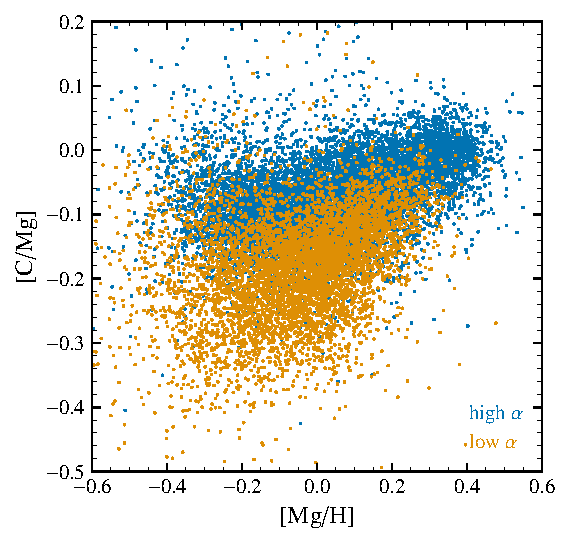
\includegraphics{subgiants_mgh.pdf}
    \quad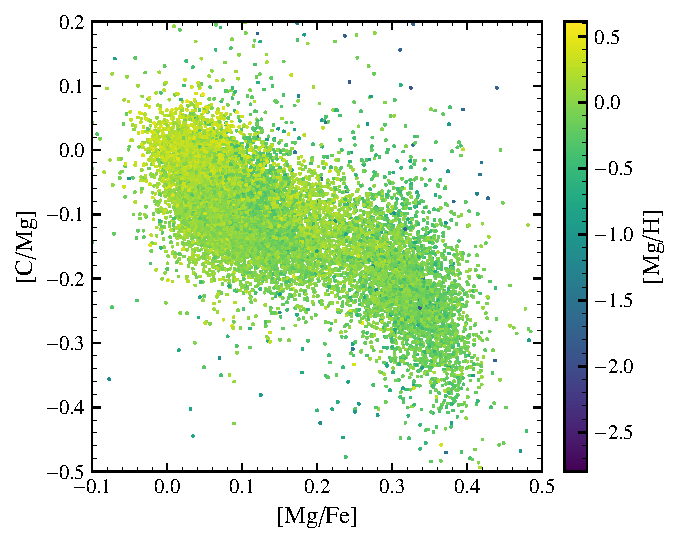
\includegraphics{subgiants_mgfe.pdf}
    \caption[Subgiant Abundances]{The [C/Mg] ratio against [Mg/H] (top) and [Mg/Fe] (bottom) for the \citetjack~sample of \apogee{} \gls{subgiant}s. On the top, I plot high and \gls{lowalpha} stars in blue and orange, using the separation defined in Equation \ref{eq:high_alpha} (the high and low-$\alpha$ stars are named for their high or low \gls{alpha} to Fe ratios, or in this case, Mg/Fe). On the bottom, I color-code stars according to their [Mg/H] abundance.}
    \label{fig:subgiants}
\end{figure}








\chapter{Nucleosynthesis}

Theoretical models of stellar \gls{nucleosynthesis} provide the starting point of this investigation. I focus on three primary nucleosynthetic pathways: \agb{} stars, \cc{}, and \ia. Each process has unique timescales and \glspl{yield}, traceable through the tools of \gce. C is produced in both \cc\ and \agb\ stars. I also compare C to Mg and Fe, which trace \cc{} and \ia{} respectively.

When a \ssp~forms, \cc{} are the first enrichment event. \Gls{cc}  explode within $\lesssim 40$\,Myr, providing light elements (C, O, and Mg) and heavier elements (Fe and beyond). O and Mg are produced almost entirely from \cc\ with metallicity-independent yields. Next, \glspl{lowmass} stars begin to reach the end of their lives. By shedding their outer layers, \agb{} stars are important sources of C, N, and neutron capture elements.  Finally, white dwarfs explode, releasing Fe and other iron-peak elements.


For an element $X$ and star with mass $M$, the net-fractional stellar \gls{yield} $\tilde{y}$ is defined as the net production of new $X$ relative to $M$, or
\begin{equation}
    \tilde{y}_{X} = \frac{M_{X,\ \rm ejected} - Z_{0, X}\,M_{\rm ejected}}{M}   
\end{equation}
where $M_{\rm ejected}$ and $M_{X, \rm ejected}$  are the total ejected mass of the envelope and the element X, respectively. For example, if a 1 $M_\odot$ star has $\tilde{y}_{\rm C} = 10^{-3}$, then the star will add $10^{-3}\ M_\odot$ of new C to the interstellar medium. 
Although per-star yields are necessary to compute \agb{} star enrichment rates in \gce{}  models, \gls{imfave} yields are useful in interpreting their predictions. For a yield $y$ from a star of mass M and initial metallicity $Z$, the \gls{imfave} yield is given by 
\begin{equation} \label{eq:imf-yield}
    y_{\rm X}(Z,t) = 
    \int_{M_{\rm min}(t)}^{M_{\rm max}} 
    \tilde{y}_{\rm X}(M, Z)
    \frac{dN}{dM}  \ dM
\end{equation}
where ${dN}/{dM}$ is the normalized \imf, $M_{\rm max}=100\,M_\odot$ is the maximum stellar mass, and $M_{\rm min}(t)$ is the mass of stars with lifetime $t$. 
\footnote{In my model, the mass-lifetime relation is
$\log \tau_M = 1.02 - 3.57\log M + 0.90 \left(\log M\right)^2$,
where $\tau_M$ is in Gyr,
from \citealt{larson74}.  For \agb{} stars, the stellar yields are truncated above 8 $M_{\odot}$. }
I use $t=10\,$Gyr for total yields when $t$ is not used.
To calculate the \gls{imfave} net yields, I use the Versatile Integrator for Chemical Evolution code (\VICE\footnote{\VICE~is available at \url{https://github.com/giganano/VICE}}).

To focus on C yields, I adapt the yield choices of other elements from \citet{james+21, james+23}.
Table \ref{tab:fiducial_mod} contains my fiducial \glspl{yield}, in units of a \ssp's birth mass.
Also following \citet{james+21, james+23}, I take the \ia{} \gls{dtd} to be a
$t^{-1.1}$ power-law suggested by the observations of \citet{maoz+12}.


\begin{table}
	\centering
    \caption[Fiducial Model Yields]{Yields for the fiducial model (in units of \ssp~birth mass). See Section \ref{sec:agb} for the definition of \cxi.}
	\label{tab:fiducial_mod}

	\begin{tabular}{l l l l}
		\toprule
        Element & $\Ycc$ & $\tilde{y}^{\rm AGB}$ & $y^{\rm SNe Ia}$ \\
		\midrule
        C & $0.0028 + 0.001(Z/Z_\odot)$ & $2.9\times{\rm C11}$ &  0 \\
        Mg & 0.00185 & 0 & 0 \\
        Fe & 0.0012 & 0 & 0.00214 \\
        N & 0.00072 & $9\times10^{-4}(Z/Z_\odot)M$ & 0\\
		\bottomrule
	\end{tabular}
\end{table}

\section{Asymptotic Giant Branch Stars}\label{sec:agb}


An \agb\ star is a \gls{lowmass} ($\lesssim 8 M_{\sun}$) during its final phase of evolution (see Appendix \ref{sec:stel_evo}).  In an \agb\ star, two competing processes determine the outcome of C production: \gls{tdu} and \gls{hbb}.  Third dredge up accompanies thermal pulses in \agb\ stars, where material from the CO core is mixed with the envelope, increasing surface C abundances \citep{KL14}. If this envelope is lost during the \agb\ phase, then C yields are enhanced.
\gls{hbb} is the activation of proton capture reactions and the CNO cycle%
at the base of the convective envelope. Because the $^{14}$N proton capture is the slowest component of the CNO cycle \citep{solar-fusion}, the CNO cycle converts nearly all \isotope[12]{C} into \isotope[14]{N}.
As a result, when both \gls{tdu} and \gls{hbb} occur, \isotope[12]{C} yields are lowered (see discussion in \citealt{james+23} and \citealt{ventura+13}).

    In this work, I explore four different sets of \agb\ star yield tables from literature, providing well-sampled grids in \gls{metallicity} and mass for use in chemical evolution models. 
\begin{itemize}
    \item \cxi: \citet{cristallo+11, cristallo+15}
    \item \kx: \citet{karakas10}
    \item \vxiii: \citet{ventura+13,ventura+14,ventura+18, ventura+20}
    \item \kxvi: \citet{KL16, karakas+18}
\end{itemize}
For my models to match observations, I find that need to uniformly amplify these yield tables (see Eq.~\ref{eq:alpha}). I use \cxi\ table, amplified by a factor of 2.9, as the fiducial \agb\ yield.

Fig.~\ref{fig:y_agb} compares the stellar \agb\ C yield $\tilde{y}_\text{C}^\text{AGB}(M, Z)$ for these four models.
The yields may be negative if a star ejects material with a lower average C abundance than the material the star was formed from.
Most models agree on the qualitative shape of the net fractional \agb\ C yield---% 
stars with masses between \about{2~M_\odot} and \about{4~M_\odot} have the highest fractional C yields, with the mass of the peak increasing and overall yields decreasing with increasing $Z$.  High mass, high $Z$ stars destroy \isotope[12]{C} because they experience both \gls{tdu} and \gls{hbb}, but the latter is much more efficient.

Fig.~\ref{fig:agb-ssp} shows the total production of C by \agb\ stars in a \ssp{} at an age $t$, i.e. $\tilde{y}_{\rm C}(Z_\odot, t)$. 
As the mass range $2M_\odot\lesssim M \lesssim 4M_\odot$ is most important for C production, about half of C production occurs before \about{1}\,Gyr, similar to \ia\ Fe. 
\kx{} and \kxvi{} weight C production more heavily towards \glspl{highmass} resulting in a faster enrichment delay time, whereas the \cxi\ and \vxiii\ models predict a slightly longer timescale of \about{1}\,Gyr, but little to no C is produced more than 2\,Gyr after a star formation event. This is in contrast to Fe whose production lasts up to 10\,Gyr after a star formation event. As shown in the right panel of Fig.~\ref{fig:agb-ssp}, with increasing $Z$, C enrichment occurs earlier, and C destruction in low-mass stars leads to a declining C abundance at late times.
    

\begin{figure}[htp]
    \centering
 	    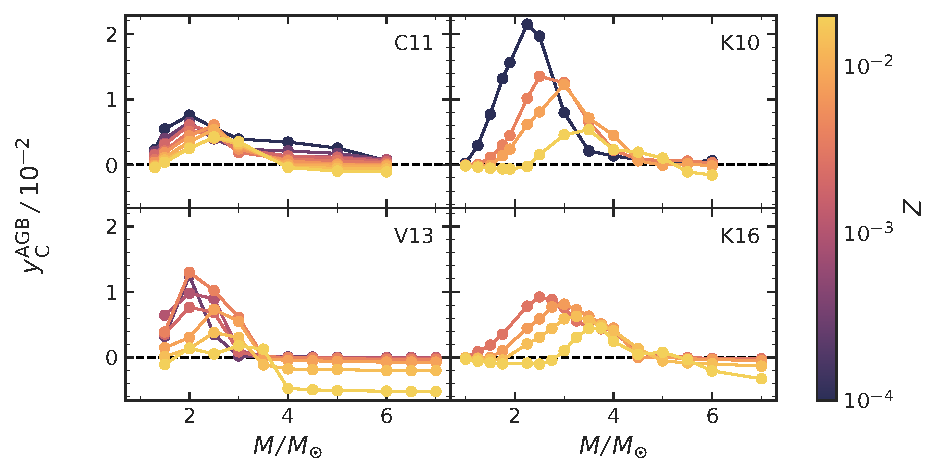
\includegraphics[scale=1]{agb_yields.pdf}
        \caption[Low-Mass Stellar Carbon Yields]{The net fractional \agb\ C yield  plotted as a function of initial stellar mass $M$ and color-coded according to metallicity. The black dashed line shows $\tilde{y}=0$ for reference. Each panel represents yields from one of four \agb\ models: \cxi, \kx{}, \vxiii{}, \kxvi{} (see Section \ref{sec:agb} and \ref{sec:oob_models}). }
        \label{fig:y_agb}
\end{figure}
\begin{figure}[htp]
    \centering
    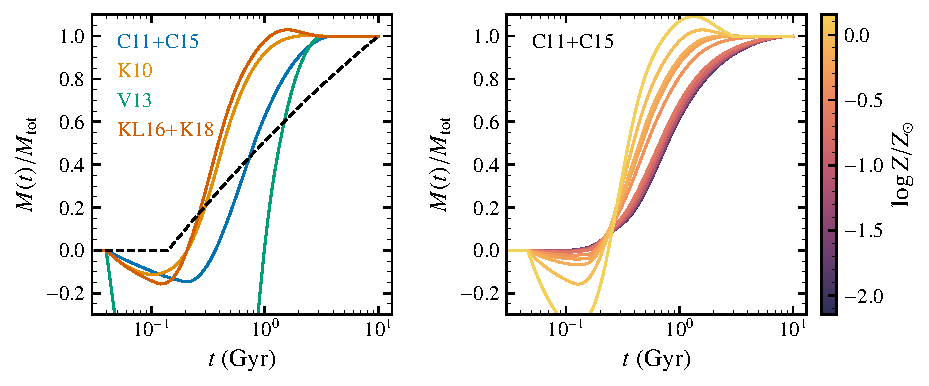
\includegraphics[scale=1]{y_agb_t2.pdf}

    \caption[Carbon Delay Time Distribution]{
    C production by \agb\ stars as a function of \ssp{} age, normalized to the total mass $M_{\rm tot}$ produced at $t=10$\,Gyr. \textbf{Left:} The four \agb\ yield models from literature at solar metallicity (\cxi, \kx{}, \vxiii{}, or \kxvi{}). The \gls{dtd} of type Ia supernovae ($\propto t^{-1.1}$) is plotted as a dashed black line for comparison. \textbf{Right:} The \cxi\ \agb\ model at different metallicities. }
    \label{fig:agb-ssp}
\end{figure}


Fig.~\ref{fig:yagb-z} shows \gls{imfave} C yields for each \agb\ model as a function of metallicity $Z$.
\vxiii{} differs in that it shows a non-monotonic metallicity dependence. However, this effect is only for models with $\log Z/Z_\odot \lesssim -1$.
Otherwise, models differ only in their yield normalization and metallicity dependence. All models predict yields within a factor of \about{2} for fixed metallicity.
For example, the three models \cxi, \kx{}, and \kxvi{} predict $y_\text{C}^\text{AGB}$ to be between 0.006 and 0.008 at solar metallicity, but \cxi\ has a much shallower metallicity dependence than the \kx{} and \kxvi{} models. \vxiii{} instead predicts a yield \about{0.004}.

\begin{figure}[htp]
    \centering
    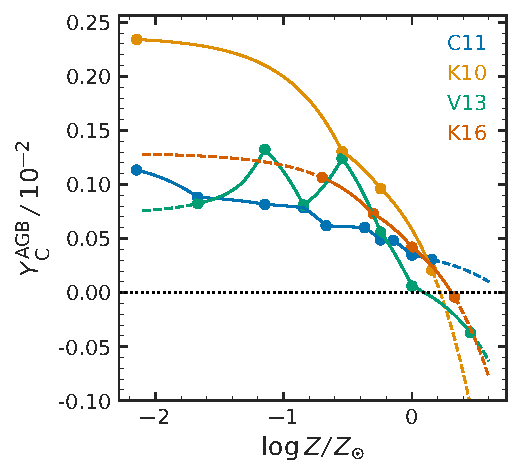
\includegraphics[scale=1]{y_agb_vs_z.pdf}

    \caption[Low-Mass-Star Yield Metallicity Dependence]{The net fractional \imf-weighted \agb\ C yield $\Ycagb$ as a function of metallicity for each of our \agb\ yield models. ($\Ycagb$ is the net mass of C produced by \agb\ stars per unit mass of star formation, after 10\,Gyr and assuming a \citet{kroupa01} \imf.)
    }
    \label{fig:yagb-z}
\end{figure}

\section{Core Collapse Supernovae}


Massive stars form $^{12}$C in their cores through the triple--$\alpha$ process (see Appendix \ref{sec:stel_evo}). However, only C ejected through supernovae and stellar winds contributes to the yield. 
While there are many stellar models providing predictions of \cc{} yields, the results of these models are highly uncertain due to the many stellar modeling uncertainties. 

Fig.~\ref{fig:y_cc} plots calculations of the \imf-integrated yields, defined with Eq.~\ref{eq:imf-yield} (computed using \VICE's \texttt{vice.yields.ccsne.fractional} function). 
\Gls{cc} models predict a wide range of C yields, spanning almost 1 dex. 
Both the \citet{NKT13} and \cite{LC18} models show positive metallicity dependence. 
The \cite{LC18} models also include rotation, showing that variations in the rotational velocity of the star can dramatically increase the magnitude and metallicity dependence of $\Ycc$. Rotation induces more mixing allowing the CO core to grow larger. As I will later show, \cc\ C production needs to be strongly metallicity-dependent at $Z/Z_\odot \approx 1$, which is consistent with the \cite{LC18} rapidly rotating models.

Fig.~\ref{fig:y_cc} shows the \cxi{} \agb\ model for comparison on the top. Especially at $Z\approx Z_\odot$, most \cc{} models dominate \agb\ C production. Later, I will also show empirically this is the case.
On the bottom of Fig.~\ref{fig:y_cc}, I also show the \cc{}-[C/Mg] ratio, defined by
\begin{equation}\label{eq:c_mg_cc}
    {\rm [C/Mg]^{CC}} = \log_{10}\left( \frac{\Ycc}{\Yoc}\right) - \log_{10} \left( \frac{Z_{{\rm C},\ \sun }}{Z_{{\rm Mg},\ \sun }} \right).
\end{equation}
${\rm [C/Mg]^{CC}}$ describes what [C/Mg] would be if \cc{} were the only process producing C.
Once again, different \cc\ models span a large range in [C/Mg]. 
I chose to instead parameterize $\Ycc$ to enable agreement with observations, as most \cc\ models fail to achieve near-solar [C/Mg].
Assumptions about the explodability landscape affect C and Mg production. Increasing the fraction of stars that explode increases $\Ycc$, as stars that directly collapse do not contribute to explosive yields \citep{emily+21}. However, C is relatively unaffected by the black-hole landscape, as very massive stars contribute C through enriched winds. Since Mg is formed deeper in the core of \glspl{highmass}, the Mg yield drops much more steeply, so models where few stars explode (S16/W18) have higher [C/Mg].

\Cc\ models also do not reach [O/Mg] due to overproduction of O or underproduction of Mg, or both \citep{emily+21}. Here, I assume ${\rm [O/Mg]} = 0$, which is not compatible with \cc\ models but is consistent with \apogee{} observations \citep{weinberg+19, weinberg+22}.
    

\begin{figure}[htp]
    \centering
    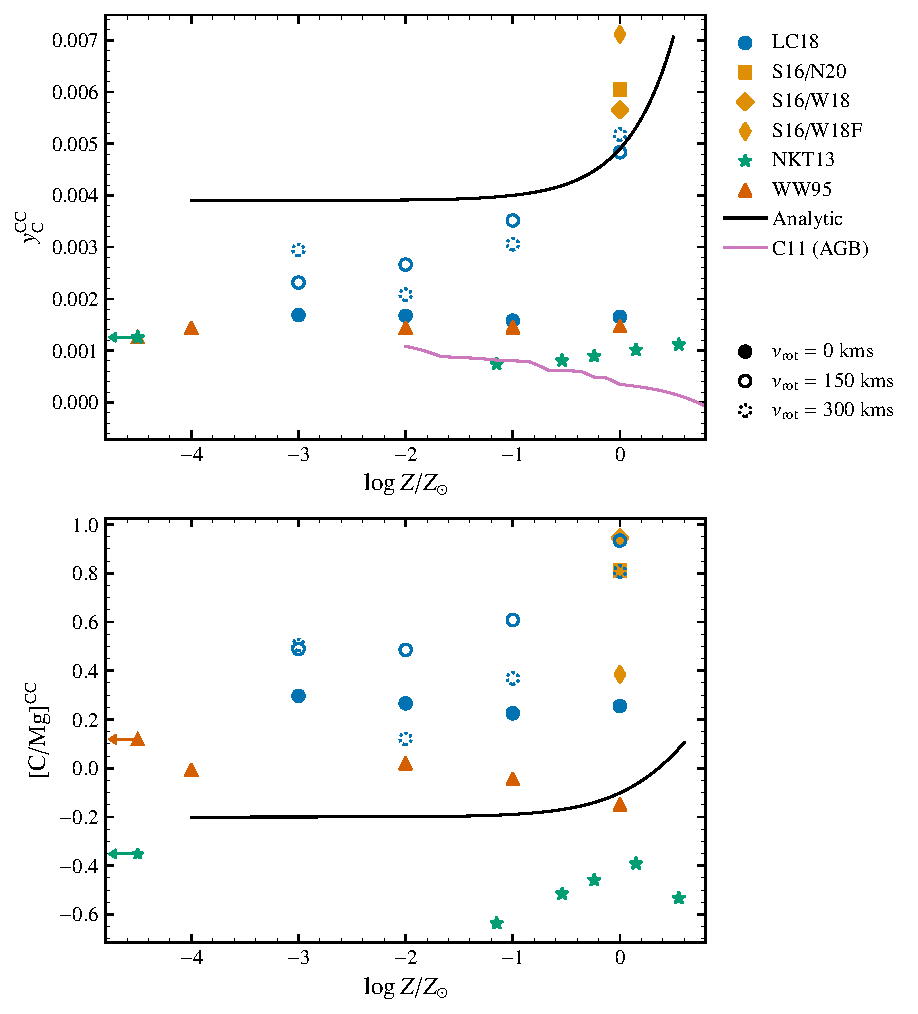
\includegraphics{y_c_cc.pdf}
    \caption[High-Mass Star Carbon Yields]{
        C yields from high-mass stars.
        \textbf{Top:} The \imf-weighted \cc\ yield of C as a function of metallicity.
        \textbf{Bottom:} The \cc\ [C/Mg] abundance ratio, defined in Eq.~\ref{eq:c_mg_cc}. The black line is the derived C yield from Section \ref{sec:equilibrium},
    $\Ycc = 0.0028 + 0.001 (Z/Z_{\odot})$. Yields are shown for tables from 
    \citet[red triangles]{WW95}, \citet[orange squares and diamonds]{sukhbold+16}, 
    \citet[green stars]{NKT13}, and \citet[blue circles]{LC18}. \citet{sukhbold+16} report yields for different black hole landscapes, while \citet{LC18} provide yields at different rotational velocities.
    In the top panel, the pink line denotes $\Ycagb$ from \cxi{} for comparison. All models include wind yields.
}
    \label{fig:y_cc}
\end{figure}

\chapter{The Equilibrium Approximation}\label{sec:equilibrium}

In the presence of metal-poor gas accretion and feedback-driven outflows, galaxies reach an equilibrium abundance in which production of new metals is balanced by losses to new stars and outflows \citep{larson72, dalcanton07, FD08, PS11, lilly13}.
While our galaxy is likely not in perfect equilibrium or described by a single, homogeneous chemical region, the equilibrium approximation is nevertheless useful in understanding yields and metallicity dependence \citep[e.g.][]{james_dwarf,james+23,WAF17}. 

I assume a simple \textit{\gls{onezone}} chemical evolution model \cite[e.g.][]{tinsley80, pagel09, matteucci21}.  Newly produced metals are homogeneously and instantaneously mixed, so spatial dependence is neglected.
I define $M_{X}$ to be the mass of element $X$ in the gas phase, $\dot{M}_\star$ to be the star formation rate (in M$_\odot$ yr$^{-1}$), and $\eta$ to be the mass loading factor $\eta\equiv\dot{M}_{\rm outflow}/\dot{M}_\star$ (representing the strength of outflows). A \ssp\ returns a fraction $r$ of their birth mass to the interstellar medium, due to ejected stellar envelopes.
\footnote{$r\approx0.4$ for a \citealt{kroupa01} \imf.}
Given the \gls{imfave} yield of Mg $y_{\rm Mg}$, the rate of change in the gas-phase mass of Mg is a simple sum of sources and sinks,
\begin{equation}
    \dot{M}_{\rm Mg} =  y_{X}\,\dot{M}_\star - \dot{M}_{\rm Mg~remnants} - \dot{M}_{\rm Mg,~outflows},
\end{equation}
where the first term on the right-hand side describes \cc\ enrichment. 
In terms of the return mass fraction of stars $r$, the mass lost to remnants is $Z_X\,\dot{M}_\star\,(1-r)$.  And, the outflows deplete mass at a rate $Z_X \,\dot{M}_\star\,\eta$. (I assume the composition of outflows is the same as the interstellar medium.) Substituting for $\eta$ and $r$,  
\begin{equation}
    \dot{M}_{\rm Mg}= y_{X} \dot{M}_\star - (1 + \eta - r) Z_{X} \dot{M}_\star.
\end{equation}
Assuming an exponentially declining star formation history $\dot{M}_\star \propto e^{-t/\tau_{\rm sfh}}$, the equilibrium abundance is derived analytically by setting $\dot{Z}_{Mg}=0$.
\begin{equation}\label{eq:z_eq}
    Z_{\rm Mg}^{\rm eq}(R) = \frac{y_{\rm Mg}}{1 + \eta(R) - r - \tau_\star / \tau_{sfh}},
\end{equation}
where $\tau_{\star}$ is the star formation rate. ($\eta$ depends on $R$ to create a metallicity gradient. See also Section \ref{sec:vice} and Eq.~\ref{eq:eta_r}.)
In the special case of constant star formation, $\tau_{\rm sfh}\to\infty$, the denominator simplifies to $1+\eta-r$.

Likewise, for \agb\ stars,
\footnote{In detail, the \agb\ contribution requires integration over the \sfh\ to account for the finite lifetimes of stars. However, for this exponential \sfh, this effect is minimal, so I simply use $\Ycagb$ for the current \agb\ contribution.}
Eq.~\ref{eq:z_eq} then becomes
\begin{equation}
    Z_{\rm C}^{\rm eq}(R) = \frac{\Ycc + \Ycagb}{1 + \eta(R) - r - \tau_\star / \tau_{sfh}}
\end{equation}
And the equilibrium C/Mg abundance ratio is
\begin{equation}\label{eq:z_co}
    \frac{Z_{\rm C}^{\rm eq}}{Z_{\rm Mg}^{\rm eq}} = \frac{\Ycc + \Ycagb }{\Yoc}.
\end{equation}
Analogous to \cite{james+23} arguments about N, the trends in abundance ratios are set by yield ratios in these \gce{} models. The effect of other \gce{} parameters (most importantly $\eta$) cancels. As a consequence, yield ratios should establish abundance ratio trends in models which assume a different normalization of element yields and mass-loading (see discussion below).
This argument can also be inverted to infer  yields from abundance ratio trends. To the extent that observed C and Mg trends reflect the equilibrium abundances in different Galactic regions, we can infer the \cc\ yield given an assumed \agb\ star yield (or vice versa). Inferring $\Ycc$ from $\Ycagb$, 
\begin{equation}
    y_\text{C}^\text{CC} =  y_\text{Mg}^\text{CC} \frac{Z_\text{C,~eq}}{Z_\text{Mg,~eq}} - \langle y_c^{agb} \rangle
\end{equation}
Rewriting this expression as a relative yield of C and Mg,
\begin{equation}\label{eq:y_c_eq}
    \frac{\Ycc}{\Yoc} = \frac{Z_{\text{C},~\odot}}{Z_{\text{Mg},~\odot}} 10^{\rm [C/Mg]} - \frac{\Ycagb}{\Yoc}.
\end{equation}

\section{Yield Models}

As I will discuss in Section \ref{sec:outflows}, the normalization of yields and $\eta$ is degenerate. This can be observed in Eq.~\ref{eq:z_co}, where changes in $\eta$ or the scaling of $y_{\rm C}/y_{\rm Mg}$ would not affect equilibrium trends. Furthermore, in Eq.~\ref{eq:z_eq}, an increase in both $y_{\rm Mg}$ and $\eta$ would leave $Z_{\rm Mg}^{\rm eq}$ unchanged. My models here are unable to distinguish the overall scaling of yields and outflow mass loading. So, choosing to keep $y_{\rm C}$ fixed reduces unnecessary free parameters. So, at solar metallicity, I set
\begin{subequations}
    \begin{align}
        \Yct~\big\vert_{Z=Z_\odot} &= \Ycc + \Ycagb = 0.005 \\
        \Yct/\Yoc~\big\vert_{Z=Z_\odot} &= 2.7.
    \end{align}
\end{subequations}
This ratio results in an equilibrium abundance ${\rm [C/Mg]} = -0.09$, which is consistent with the \citetjack~\gls{subgiant} sample and is within \about{20\%} of the solar C/Mg mixture from \citet{asplund+09}.

In Section \ref{sec:f-z-models}, I will show that none of the four \agb\ yield sets (\cxi{}, \kx{}, \vxiii{}, \kxvi{}) produce enough C relative to this $\Ycc$ value. So, I introduce normalization factors, $\alpha_{\rm AGB}$, and $\alpha_{\rm CC}$ which denote a multiplicative scaling of $\Ycc$ and $\Ycagb$ respectively. 
\begin{subequations} \label{eq:alpha}
    \begin{align}
        \Ycagb &\rightarrow \alpha_{\rm AGB}\ \Ycagb \\
        \Ycc &\rightarrow \alpha_{\rm CC}\ \Ycc\\
        \alpha_{\rm CC} &= \frac{\Yct - \alpha_{\rm AGB}\ \Ycagb}{\Ycc}
    \end{align}
\end{subequations}
Above, $\alpha_{\rm CC}$ is dependent on the choice of $\alpha_{\rm AGB}$ to keep the total C yield constant. 

In Section \ref{sec:f-z-models}, I find that $\alpha_{\rm AGB}\approx 2.9$ for the \cxi{} yield model. Using this \agb\ yield, I can now use Eq.~\ref{eq:y_c_eq} to find an estimate of $\Ycc$ as a function of metallicity. I show the values of $\Ycc$ I obtain from the \gls{subgiant} sample in Fig.~\ref{fig:analytic}. From a regression analysis, I suggest here that
\begin{equation}\label{eq:zeta}
    \Ycc = 0.0028 + \zeta\left(\frac{Z}{Z_\odot}\right),
\end{equation}
where $\zeta\approx.001$ describes the metallicity dependence.


\begin{figure}[htp]
    \centering
    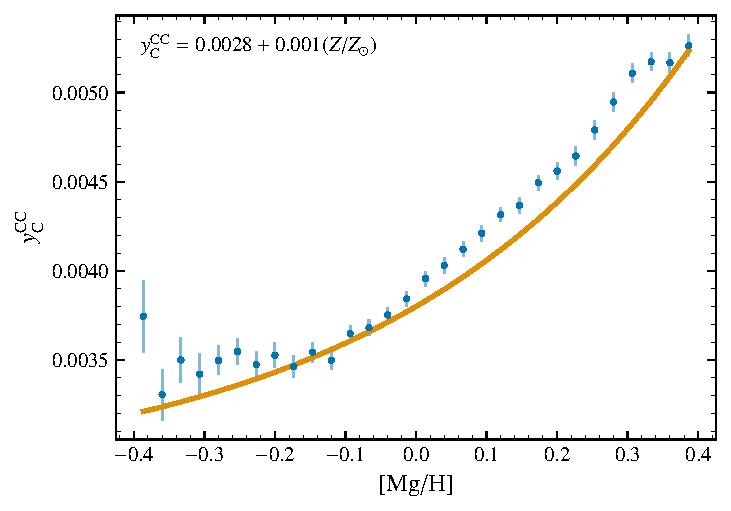
\includegraphics[]{analytic.pdf}
    \caption[Reverse-Fit Yields]{Inferred high-mass star C yields as a function of metallicity. I assume equilibrium and $3\times {\rm C11}$ \agb\ yields (orange curve, see discussion in Section \ref{sec:equilibrium}). Blue points are the median value of $\Ycc$ for each bin in [Mg/H] with uncertainties based on the median absolute deviation.
    }
    \label{fig:analytic}
\end{figure}





\section{Uncertainties}

I only perform this analysis on the \cxi{} yields because \cxi{} has yields tables more finely sampled in metallicity than the other three \agb\ yield tables. As the metallicity range of the data is small ($-0.4\lesssim {\rm [Mg/H]} \lesssim 0.4$), other models are more challenging to interpret in this range. Furthermore, the \apogee{} observations may have systematics, and other measurements of C abundances \citep[e.g.][]{vincenzo+21} have slight disagreements in the overall shape of the trend (see Section \ref{sec:jack}).
So, this expression of $\Ycc/\Yoc$ depends on the chosen \agb\ yield table, the \agb\ fraction, and the dataset. 
Additionally, these yields will be systematically biased if the galaxy is out of equilibrium, for example, due to a recent starburst (Isern et al. 19; Mar et al. 19). Further exploration could investigate the magnitude of these uncertainties, but I find that the qualitative conclusions are similar despite substantial variations in the assumptions here.



\chapter{The Multizone Model}\label{sec:vice}

Classical, \textit{\gls{onezone}} models of chemical evolution assume instantaneous mixing of metals in the star-forming interstellar medium \citep[e.g.][]{matteucci21}. This simple framework is a poor approximation of the Milky Way.  The Galaxy evolves \gls{insideout}---where star formation is higher towards the center and in the early universe \citep{bird+13}. Additionally, stars can migrate several kpcs over their lifetimes, mixing different chemical environments across the galaxy \citep{bird+12,sellwood+binney02}. For the rest of this paper, I focus on \gls{multizone} models, which discretize the Galaxy into concentric rings in which stars move between.  Specifically, I make use of the \citet{james+21} (hereafter \JJ) model for the Milky Way, which runs using the publicly available Versatile Integrator for Chemical Evolution (\VICE). This model is described extensively in \JJ~and concisely summarized  in \citet{james+23}. Here, I provide a brief overview of the relevant model components.

In the model, the Galaxy is divided into 200 rings, each 100 pc wide. Each ring has a separate stellar population and gas supply. Star formation ends beyond a radius $R=15.5$ kpc. I initially assume an \gls{insideout} \sfh{}, where the star formation surface density $\Sigma_\star$ is given by 
\begin{equation}\label{eq:inside_out}
    \dot{\Sigma}_\star \propto \left(1-e^{-t/\tau_{\rm rise}}\right) e^{-t/\tau_{\rm sfh}}.
\end{equation}
$\tau_\text{rise}=2$\,Gyr describes when the star formation rate reaches a maximum, and $\tau_{\rm sfh}$ describes the decay timescale of star formation as a function of radius $R$. \JJ~derives $\tau_{\rm sfh}(R)$ through analysis of four integral field spectroscopy surveys in \cite{sanches20}. The star formation history is normalized such that the total stellar mass reaches $5.17\times10^{10} {\rm M}_\odot$ \citep{LM15} and at each $R$ to match the stellar surface density gradient \citep{BHG16}.
The gas inflow is calculated to maintain our chosen \sfh{} for each radius and time. The gas-star-formation law is based on an extension of a Kennicutt-Schmidt law \citep{kennicutt98}
\begin{equation}
\dot{\Sigma}_{\star} \propto 
\begin{cases}
    {\Sigma}_{\rm gas} & 2\times 10^7 \leq \Sigma_{\rm gas} \\ 
    {(\Sigma}_{\rm gas})^{3.6} & 5\times 10^6 \leq \Sigma_{\rm gas} < 2\times10^7 \\ 
    {(\Sigma}_{\rm gas})^{1.7} & \Sigma_{\rm gas} < 5\times10^6 \\ 
\end{cases}
\end{equation}
The scaling of this relationship varies with time due to the redshift dependence of $\tau_\star$ in molecular gas observed by \citet{tacconi18}. I assume a \citet{kroupa01} \imf.


\JJ\ accounts for radial migration by using the results of the \texttt{h277} hydrodynamical simulation \citep{christensen12, zolotov12, loebman12, BZ14}, with simulation parameters described in \citet{bird+21}. Each \VICE\ single stellar population (SSP) is matched to an \textit{analog} in \texttt{H277}, chosen to form at a similar time and radius $R$. By taking the change in radius $\Delta R$ of the analogs, the \ssp move to their final radii with a $\sqrt{\text{time}}$ dependence.
This relationship between displacement and time arises when migration proceeds as a consequence of the diffusion of angular momentum \citep{frankel18, frankel20}.
I do not account for radial gas flows.
Using the results of a hydrodynamical simulation without modification limits the free parameters in the model; however, I am limited to one dynamical history. The impact of the details of a galaxy's dynamical history on its chemical evolution is unknown.

As the strength of outflows controls the resulting $\alpha$ abundances, \JJ~create a metallicity gradient by defining
\begin{equation}\label{eq:eta_r}
\eta(R) = \frac{y_{\alpha}^{\rm CC}}{Z_{\alpha, \odot}} 10^{(-0.08\text{ kpc}^{-1})(R-4\text{ kpc})+0.3} + r - 1.
\end{equation}
This choice of $\eta(R)$ results in a [$\alpha$/H] gradient consistent with Milky Way observations \citep[e.g.][]{hayden+14, weinberg+19, frinchaboy+13}.


\chapter{Multizone Model Results}
\section{Data Selection}

\citet{james+23} compare their model against the \cite{vincenzo+21} sample of \apogee{} \citep{apogee17} \gls{rgb} stars. \citet{vincenzo+21} use \textsc{mesa} stellar evolution models \citep{mesa} to correct for the effects of \gls{fdu}. 
I instead use the \citetjack~sample of \apogee{} \gls{subgiant}s. Subgiant stars have not undergone \gls{fdu} but have well-mixed atmospheres, so their atmospheric C and N abundances are still reflective of their birth abundances and do not need mixing corrections. I only compare the models to the \gls{lowalpha} sequence unless otherwise specified.  The selection criteria and differences between the samples are described in more detail in Appendix \ref{sec:jack}.



\section{The Evolution of C Abundances in the Galaxy}

Here, I present the time evolution of our fiducial model. In the next Sections, I will discuss the choice of parameters and agreement with observations. 
The fiducial model has the following qualitative characteristics of its C yields: (a) C is predominantly produced in \cc, (b) \cc\ produce more C at higher metallicities, and (c) \agb\ stars produce less C at higher metallicities. The fiducial model uses the \cxi{} \agb\ yield tables (see Section \ref{sec:agb}, and Table \ref{tab:fiducial_mod}), and I amplify the \cxi{} yields by a factor of 2.9 such that \agb\ stars account for 20\% of C at $Z=Z_\odot$. 

I show the time evolution tracks of the fiducial model in Fig.~\ref{fig:c_evo} for \caah~ and \caafe. Comparing [C/Mg] against [Mg/Fe] enables us to see the late-time evolution of C more clearly. Because of the extended \gls{dtd} of \ia\ enrichment, [Fe/H] takes longer to reach equilibrium, and the late-time evolution is not as clustered as [Mg/H].
The evolution proceeds as follows.
Initially, \cc\ dominate production. As $\Ycc$ has strong metallicity dependence, [C/Mg] increases with time. Shortly thereafter, \agb\ stars contribute delayed C, increasing [C/Mg] even more steeply. As Mg begins to reach equilibrium, the [C/Mg] ratio plateaus as C approaches equilibrium. Finally, as $\Ycagb$ decreases or even becomes negative with higher metallicity, the [C/Mg] abundance may decline slightly. 
This is even more evident in the lower panel of Fig.~\ref{fig:c_evo}. While the \caah\ trend reaches equilibrium at \about{5}\,Gyr, the \caafe\ trend continues to evolve even until the present day, exposing the effect of the relative delay times of \agb\ stars and \ia.


\begin{figure}[htp]
\centering
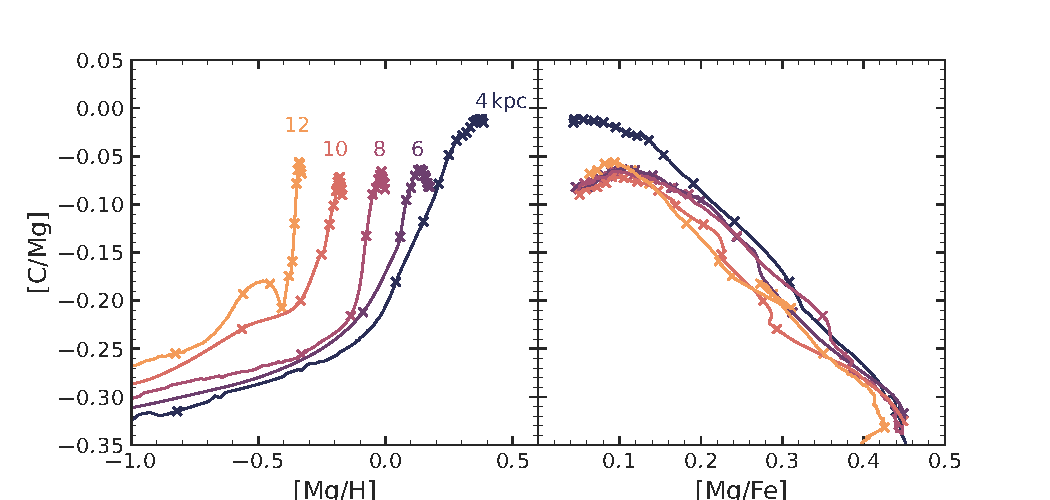
\includegraphics{evo_tracks.pdf}
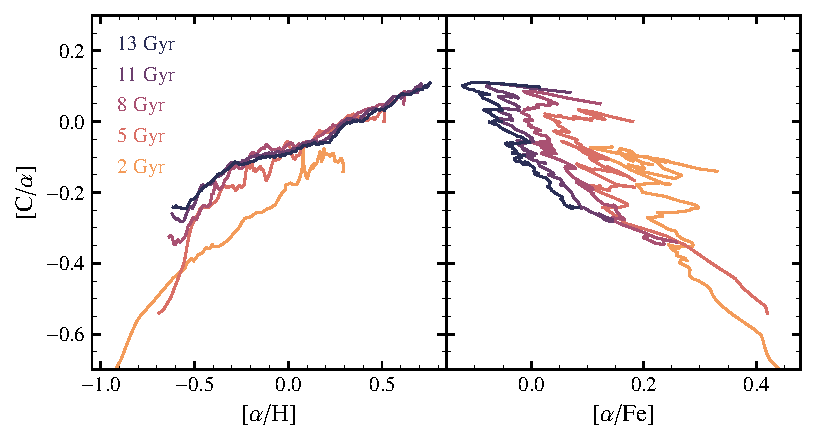
\includegraphics{evo_slices.pdf}
\caption[Carbon Chemical Evolution Tracks]{
    Time evolution of gas phase C abundances in our fiducial model.
    {\bf Top:} Evolutionary tracks parameterized by time at fixed Galactocentric radius in the \caah\ and \caafe\ planes. 
    {\bf Bottom:} snapshots of the gas-phase \caah\ and \caafe\ trend, parameterized by radius at a fixed time.
}
\label{fig:c_evo}
\end{figure}

\section{Low and High-Mass Stellar Yields}\label{sec:f-z-models}

To parameterize the \agb\ contribution to C production, I define 
\begin{equation}\label{eq:f_agb}
    f_{\rm AGB} \equiv \frac{\Ycagb}{\Yct}\Bigg\vert_{Z=Z_\odot},
\end{equation}
where  $\Ycagb$ includes the multiplicative factor $\alpha_{\rm AGB}$ as defined in Eq.~\ref{eq:alpha}.
Fig.~\ref{fig:agb_sims} compares the \kx{}, \kxvi{}, \cxi{}, and \vxiii{} yield models. I use the published, unscaled yield tables ($\alpha_{\rm AGB}=1$) for Fig.~\ref{fig:agb_sims}. As the highest \agb\ yield at solar, \kx{} is only $\Ycagb=0.000585$, $f_{\rm AGB} \leq 0.12$ for all models. Massive stars dominate C production with unscaled yields.  While it is easy to modify the \agb\ yields in my model, their small contribution reduces the effect. I leave a more detailed discussion of the effects of \agb\ models for Appendix \ref{sec:alt_agb} and use \cxi{} yields hereafter.

\begin{figure}[htp]
\centering
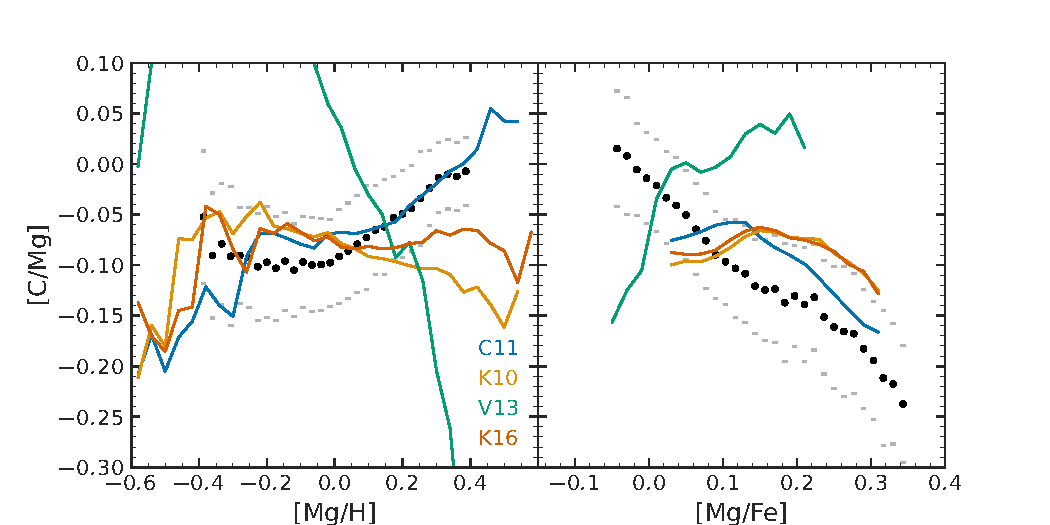
\includegraphics{agb_oob.pdf}
\caption[Median Stellar Abundance Trends]{
    Stellar abundance trends in our model, assuming metallicity independent $\Ycc$. Colored lines quantify the median [C/Mg] in bins of [Mg/H] for our four \agb\ yield models from the literature (see \ref{sec:agb}). Black points and grey dashes represent the median and standard deviations of [C/Mg] for each [Mg/H] bin in the \citetjack~sample. In the right panel, I show the trends only for stars where $-0.15\leq {\rm [Mg/H]}\leq -0.05$.
}
\label{fig:agb_sims}
\end{figure}


Next, I investigate adjustments to the \agb\ yield fraction $f_{\rm AGB}$ and the \cc\ metallicity dependence $\zeta$ in Fig.~\ref{fig:beta_f}. On the top panel of Fig.~\ref{fig:beta_f}, I plot models with varying $\Ycc$ metallicity dependence. As discussed in Section \ref{sec:equilibrium}, the \caah~trend is approximated by equilibrium, so the trends of these have steeper \caah~corresponding to steeper metallicity dependence. However, \caafe~is minimally affected by these changes since \cc\ occurs on much shorter timescales than \ia\ and \agb\ enrichment.

In the bottom panel of Fig.~\ref{fig:beta_f}, I plot three models with different \agb\ fractions while using \cxi{} yields.  The \caafe~relationship is set by $f_{\rm AGB}$ because a specific amount of C must be released at a delayed time to match the \ia\ production of Fe and increase [C/Mg] as [Mg/Fe] decreases to reproduce the data.
Increased $f_{\rm AGB}$ results in a decreased slope in \caah, owing to the negative metallicity dependence of $\Ycagb$. So while \caah~alone cannot differentiate models which vary $f_{\rm AGB}$ and $\zeta$ correspondingly, \caafe~provides information on $f_{\rm AGB}$. So, I can use \caafe~to estimate $f_{\rm AGB}\approx 0.2$, and then choose $\zeta$ to match \caah.

One source of theoretical uncertainty in this result is that the \ia\ yield and \gls{dtd}s have their own uncertainties. I discuss variations in $y_{\rm Fe}^{\rm Ia}$ in Appendix \ref{sec:alt_agb}, and find that the qualitative conclusions are largely unaffected. I, therefore, focus on the choices of $y_{\rm Fe}^{\rm Ia} = 0.00214$ and a $t^{-1.1}$ \gls{dtd} choices from the fiducial model here.
In short, the scaling of the trend and metallicity dependence of C (as seen in
the \caah\ trend) gives information on the total C yield and the behavior of \cc\ (as the dominating producer of C), the \caafe\ trend exposes the delayed effect of C from \agb\ contribution.

\begin{table}
	\centering
    \caption[Low-Mass Stellar Carbon Yields at Solar Metallicity]{For each \agb\ yield set, the \gls{imfave} \agb\ C yield at solar metallicity $y_{\rm C, 0}^{\rm AGB}$ and the multiplicative factor reaches an \agb\ contribution of 20\% $\alpha_{\rm AGB, 20}$.}
	\label{tab:alpha_agb}
	\begin{tabular}{ccr} % four columns, alignment for each
		\toprule 
		AGB Model & $y_{\rm C, 0}^{\rm AGB}$ & $\alpha_{\rm AGB, 20}$\\
        \midrule
        \cxi & 0.000347 & 2.9\\
        \kx & 0.000585 & 1.7\\
        \vxiii & 0.000060 & 16.5\\
        \kxvi & 0.000421 & 2.4\\
		\bottomrule
	\end{tabular}
\end{table}


\begin{figure}[htp]
\centering
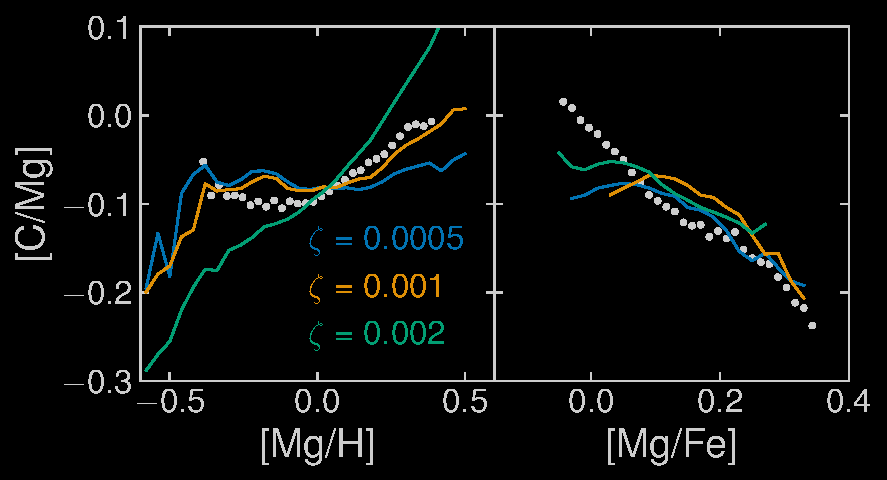
\includegraphics{beta.pdf}
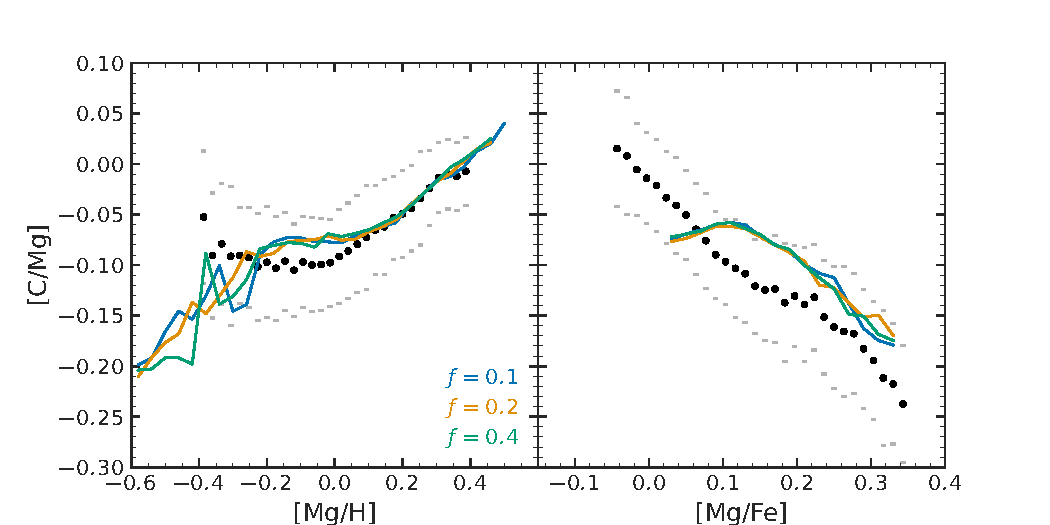
\includegraphics{f_agb.pdf}

\caption[Adjusted Yield Models]{Similar to Fig.~\ref{fig:agb_sims} except the top plot shows the fiducial model with lower and higher values of $\zeta$, the metallicity dependence of $\Ycc$. The bottom plot shows models with $f_{\rm AGB}=$0.1, 0.2, and 0.4. Both the $f_{\rm AGB}$ and $\zeta$ influence \caah, but only $f_{\rm AGB}$ has a significant impact on \caafe.}
\label{fig:beta_f}
\end{figure}



\section{Star Formation History} \label{sec:sfh}


\begin{figure}[htp]
\centering
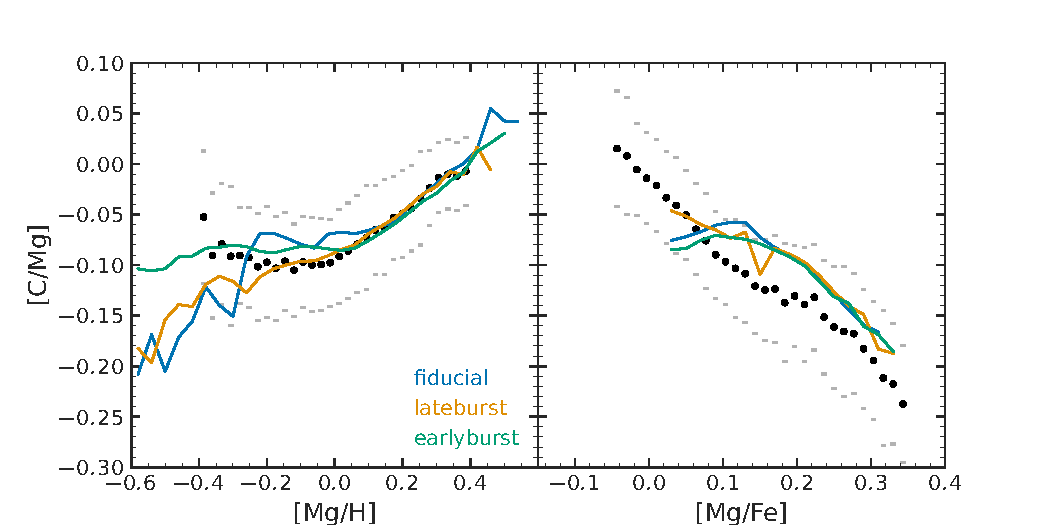
\includegraphics{lateburst_eta.pdf}

\caption[Alternate Star-Formation-History Models]{Similar to Fig.~\ref{fig:agb_sims} but comparing the fiducial model to alternate \glspl{sfh} (see Section  \ref{sec:sfh}).}
\label{fig:sfh_models}

\end{figure}


Here, I consider a \textit{lateburst} model, created by multiplying our fiducial \gls{insideout} \sfh{} with a Gaussian.
\begin{equation}\label{eq:lateburst}
    \dot{\Sigma}_{\rm lateburst} \propto \dot{\Sigma}_{\rm insideout} \left(1 + A\,e^{-(t-\tau_{\rm burst})^2/2\sigma^2_{\rm burst}} \right)
\end{equation}

$A=1.5$ represents the amplitude of the birth, $\tau_\text{burst}=10.8$\,Gyr is the time where the burst is strongest, and $\sigma_\text{burst}=1$\,Gyr is the width of the burst.
I also consider an \textit{earlyburst} model as a slight variation of the lateburst, where the burst is instead exponential and placed at $t_1=5$\,Gyr. 
\begin{equation}\label{eq:twoinfall}
    \dot{\Sigma}_{\rm earlyburst} \propto \dot{\Sigma}_{\rm insideout} + 
\begin{cases}
    A\,e^{-(t-t_1)/\tau_{\rm burst}} & t_1 < t \\
      0 & t<t_1
\end{cases}
\end{equation}
where I take the burst duration, $\tau_{\rm burst}=1$\,Gyr in this case. 
This approximately corresponds to the Gaia-Encelidus merger, inducing higher star formation in the Milky Way \citep{spitoni21, bonaca20, helmi18}.

Fig.~\ref{fig:sfh_models} shows three models with these alternate \sfh{}. Changes to the \sfh{} leave \caah\ unchanged, but they do introduce slight variation in \caafe. Models with higher \agb{} fractions are more sensitive to variations in the \sfh{}. The late burst models result in [C/Mg] continuing to increase at low [Mg/Fe], but also introduce a dip not present in the data. Additionally, the early burst
reproduces the slight break between the low and high $\alpha$ sequences, but overshoots equilibrium more severely than the fiducial model. 
In general, any of these \sfh{}s are consistent with this model.

\section{Outflows} \label{sec:outflows}

\Gce{} models of the Milky Way fall into two classes---those which incorporate significant mass-loading (e.g., as in this work) and those which neglect mass-loading but lower effective yield to match observed abundances \citep[e.g.][]{MCM13, MCM14, spitoni19, spitoni20, spitoni21}.
An increase in stellar yields has a nearly identical effect as a decrease in the mass-loading factor $\eta$ (see Appendix B of \citealt{james_dwarf}).
The equilibrium arguments discussed in Section \ref{sec:equilibrium} suggest however that abundance ratios are independent of the choice of normalization and the value of $\eta$. I, therefore, expect my results regarding the relative yield $y_{\rm C}/y_{\rm Mg}$ and its metallicity dependence to extend to the other class of models omitting mass loading. I demonstrate this further here.

The theoretical motivation for decreasing yields is the uncertainty in stellar explodability.
If fewer \glspl{highmass} explode, then the yields will be reduced by some factor. Additionally, some fraction of SN ejecta may be lost directly to an outflow, lowering effective yields. To explore reduced outflow models, I lower both $\eta$ and all yields by the same factor to leave the equilibrium abundances unchanged. 

Fig.~\ref{fig:eta} shows models with variations of the mass loading strength. While changing the value of $\eta$ affects the metallicity distribution of stars, all of the models in Fig.~\ref{fig:eta} still evolve along the same path. My model is unable to differentiate a uniform decrease in both outflows and yields.

\begin{figure}[htp]
    \centering
    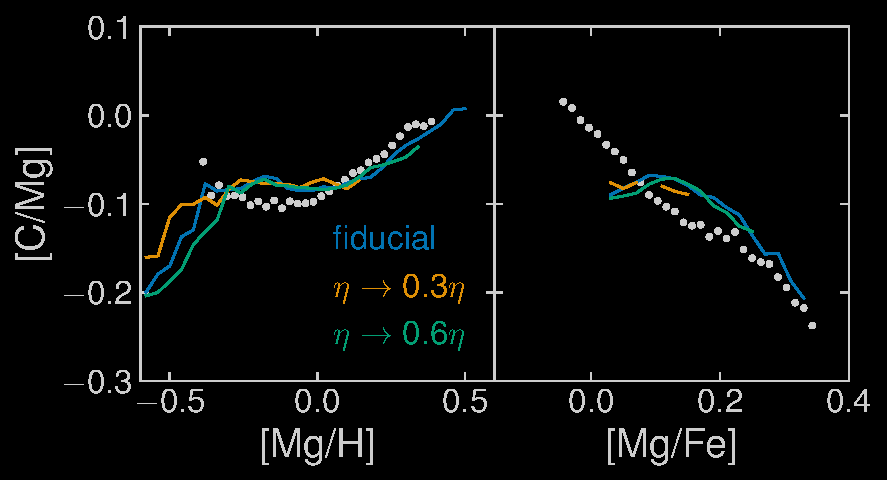
\includegraphics{eta.pdf}
    \caption[Reduced-Outflow Models]{Similar to Fig.~\ref{fig:agb_sims} but comparing the fiducial model to reduced mass loading models (see Section  \ref{sec:outflows}). Both yields and mass-loading are adjusted correspondingly such that the equilibrium abundances are unchanged. }
    \label{fig:eta}
\end{figure}


\section{Scatter}

Median trends have limitations as they do not consider the actual distribution of \caah~abundances. So, I show in Fig.~\ref{fig:scatter} a comparison of the predicted distribution of the model to the contours of the \gls{subgiant} sample. The model reproduces this 2-dimension distribution well when including scatter based on the median \apogee{} abundance errors for each metallicity bin. Some scatter is due to radial migration, but observational errors are dominant. Precision abundance measurements will allow tighter constraints on relative yields. 

\begin{figure}[htp]
    \centering
    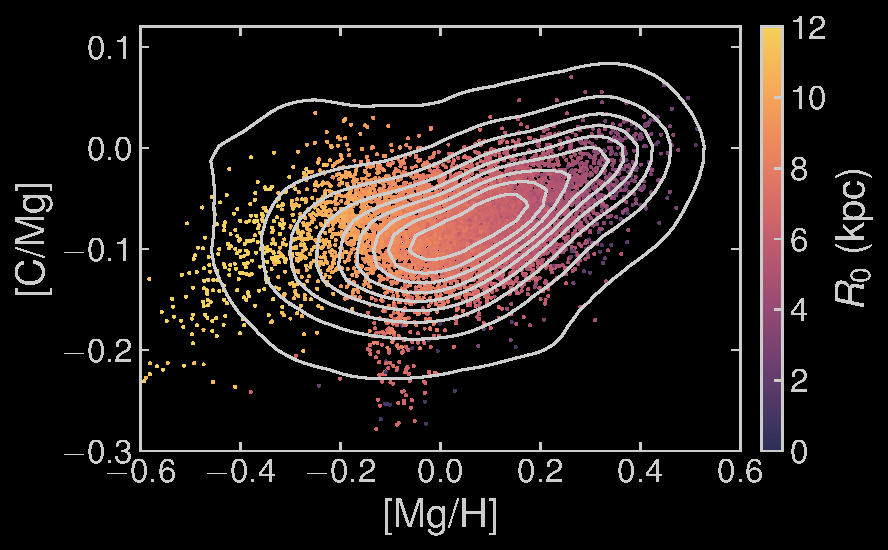
\includegraphics[scale=0.9]{cooh_scatter.pdf}
    \caption[Scatter Agreement]{The stars in the fiducial model in the \caah~plane compared to contours of the \gls{subgiant} sample. I added random noise to the scatter points equal to the median uncertainties in the \gls{subgiant} sample. Stars are color-coded such that lighter colors represent populations born at greater galactocentric radii. The plot only includes \gls{lowalpha} stars.
    }
    \label{fig:scatter}
\end{figure}



\section{Gas-Phase Abundances}\label{sec:gas}

As an additional test of the model, I next compare the model predictions against gas-phase measurements. Fig.~\ref{fig:gas_phase} shows the fiducial model's gas phase predictions compared to observations of the Milky Way and extragalactic HII regions, halo stars, and \dla\ systems. The model is broadly consistent with observations, where the model at $t=2$\,Gyr approximates the slope of dwarf galaxies and halo stars. The increase of C/O at higher metallicities is also consistent with the high C/O abundances measured in extragalactic HII regions. 
My model does not extend to very low metallicity, where the slope of the trend inverts, but broadly explains observations above $\rm [O/H] \gtrsim -1$. 

Mg measurements are more reliable, but O abundances are easier to measure in HII regions. So while I use Mg as the representative \gls{alpha} for stellar abundances, I instead use O when comparing gas-phase abundances. As I assume ${\rm[Mg/O]}=0$, my model is independent of the choice of the \gls{alpha}

Measurements of C abundances in the gas-phase are challenging. In HII regions, C/O abundance ratios are measured with either recombination lines or collisional excitation lines. However C lacks strong collisional excitation lines, and recombination lines fall in the ultraviolet without nearby reference H lines \citep{skillman+20}. Additionally, recombination and collisional excitation measurements disagree by a factor of \about{2} \citep{GR07}.
Variations in the \sfh{}s may furthermore increase scatter, as \agb\ are a delayed source of C.

The decreasing [C/O] abundance at very-low metallicities is likely due to population III stellar yields \citep[e.g.][]{hirschi07}, as suggested by \citet{cooke+17} and \citet{FN15}. \Gls{agb} stars cannot explain the increase in C yields at low metallicity in the \dla{} sample as the evolutionary timescales of \dla{}s are shorter than the typical delay time distribution of \agb\ stars.

\begin{figure}[htp]
    \centering
    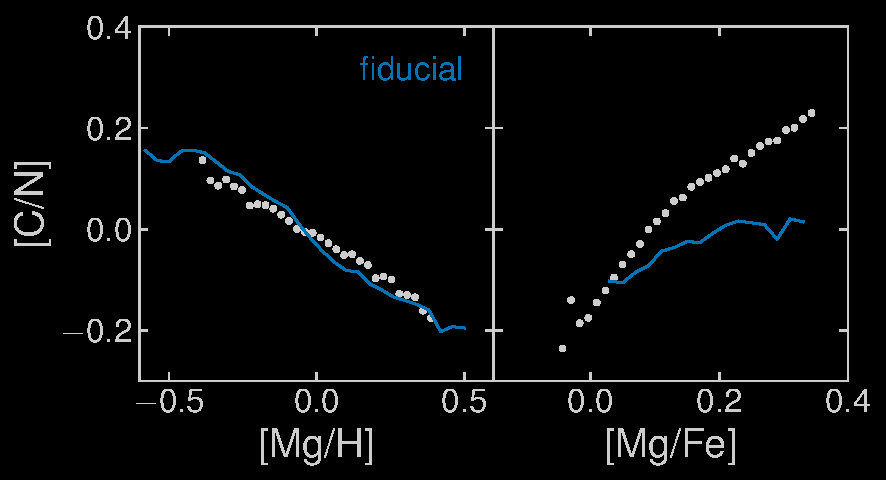
\includegraphics{c_n.pdf}
    \caption[C/N Abundance Agreement]{Similar to Fig.~\ref{fig:agb_sims}, except comparing [C/N] from the fiducial model only. N yields are adapted from \cite{james+23}. (See also Table \ref{tab:fiducial_mod}.)
    }
\end{figure}

\begin{figure}[htp]
\centering
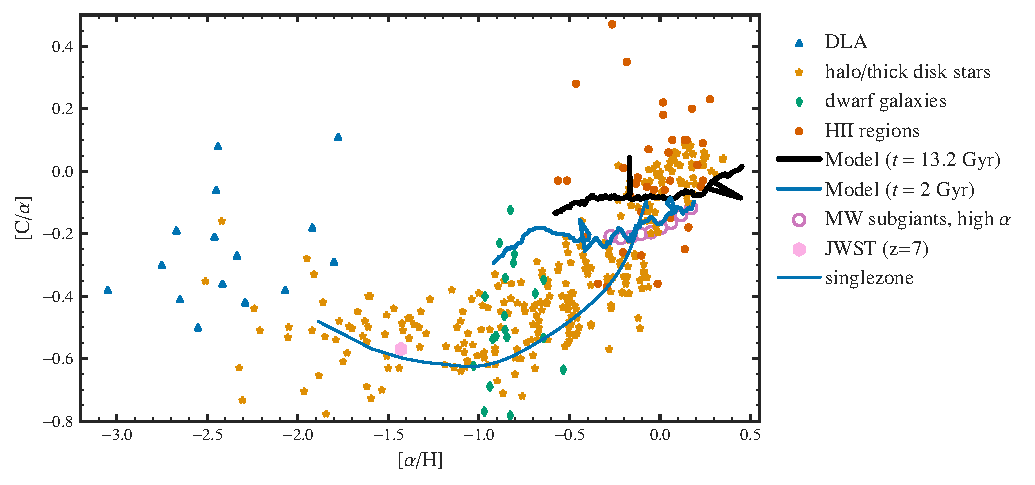
\includegraphics[]{summary.pdf}
\caption[Gas-Phase Abundances]{Gas-phase C abundances. We plot our model at $t=2$\,Gyr and present day as thick solid lines. Points represent measurements in 
    HII regions    \citep[pink circles;][]{skillman+20, esteban+02, esteban+09, esteban+14, esteban+19}
    \dla\ systems \citep[blue triangles;][]{ellison+10, srianand+10, dutta+14, DZ+03, pettini+08, morrison+16,cooke+17},  % a1: Cooke et al. (2015); 2: Dutta et al. (2014); 3: Cooke et al. (2014); 4: Ellison et al. (2010); 5: Cooke et al. (2011b); 6: This work; 7: Pettini et al. (2008); 8: Morrison et al. (2016); 9: Srianand et al. (2010); 10: Cooke et al. (2012); 11: Dessauges-Zavadsky et al. (2003)
    dwarf galaxies \citep[red diamonds;][]{berg+19},
    Milky Way halo and thick disk stars \citep[green stars;][]{nissen+14, fabbian+09},
    and Milky Way \gls{highalpha} stars (yellow points; \citealtjack).
}
\label{fig:gas_phase}
\end{figure}


\chapter{Conclusions}

In this work, I investigate the role of C yields on the predictions of \gls{multizone} \gce{} models. \citet{james+23} performed a similar analysis focusing on N. They found that matching the observed relationship between N and O abundances \citep{HEK00,PVT10,berg+12, berg+20, skillman+20, izotov+12, james2+15, dopita+16} requires relative N and O yields from simple stellar populations with a roughly linear dependence on metallicity (i.e. $y_{\rm N}/y_{\rm O} \propto Z$). 
Here, I perform a similar analysis on C. 

Though \cc\ C yields are poorly understood, I adopt an equilibrium approximation and determine a functional form that approximately matches trends in \apogee{} \gls{subgiant} and is consistent with \gls{highmass} \gls{nucleosynthesis} models. Variations of the metallicity dependence of this \cc\ yield affect trends in \caah~but do not affect trends in \caafe\ (when taking a slice in [Mg/H]). As all theoretical \agb\ C yields decrease with metallicity, increasing the \agb\ fraction causes the \caah\ trend to flatten. However, the \caafe\ trend is sensitive to the \agb\ fraction. 
From this, I estimate that \agb\ stars contribute \about{20\%} of total C abundance at solar metallicity. The remaining \about{80\%} of C comes from \gls{highmass} with a metallicity dependent yield of $\Ycc/\Yoc=1.51 + 0.54 (Z/Z_\odot)$. 
This metallicity dependence is roughly consistent with rotating stellar yields.
 

I additionally explore variations of the assumed \sfh{} and outflow mass-loading factor $\eta$. I find that alternate \sfh{}s can slightly affect \caafe, but \caah~is mostly unaffected. Decreasing both outflows and yields by the same factor leaves the \caah~and \caafe~trends unaffected. These constraints on the relative yields of C, O, and Mg are robust against variations in $\eta$.

Finally, I compare my model against gas phase measurements and metal-poor stars. While my model was built on data near solar metallicity, observations of very low metallicity, high redshift damped Lyman-$\alpha$ systems indicate higher C/O ratios \citep{cooke+17}, consistent with yields from population III stars \citep[e.g.][]{hirschi07}. Population III stars, \cc\, and \agb stars altogether explain the observed evolutionary history of C.

These C yield constraints provide a useful benchmark for stellar evolution models. C yields are sensitive to poorly understood processes, including mass loss prescriptions, explodability, nuclear cross Sections, convection, and stellar structure. Future spectroscopic surveys combined with Gaia kinematics \citep{gaia} will continue to enhance our understanding of chemical evolution. Both the Sloan Digital Sky Survey V's Milky Way Mapper program ({\sc SDSS-V/MWM}) \citep{sdssv} and the Dark Energy Spectroscopic Instrument ({\sc DESI}) Milky Way survey \citep{desi, desi:mw} will each measure spectra of upwards 6,000,000 Milky Way stars. These larger samples will enable similar work to tighten constraints on stellar models and our understanding of galaxy structure and evolution.


%%%%%%%%%%%%%%%%%%%% REFERENCES %%%%%%%%%%%%%%%%%%

\newpage
\bibliographystyle{aasjournal}
\addcontentsline{toc}{chapter}{Bibliography}
\bibliography{main} 


%%%%%%%%%%%%%%%%% APPENDICES %%%%%%%%%%%%%%%%%%%%%

\appendix
% \chapter*{Appendix}
% \addcontentsline{toc}{chapter}{Appendix}
% \renewcommand{\thesection}{A.\arabic{section}}
% \renewcommand\thefigure{A.\arabic{figure}}    
% \renewcommand\theequation{A.\arabic{equation}}    
% \setcounter{figure}{0}
% \setcounter{equation}{0}
% 
% \renewcommand*{\theHsection}{A.\arabic{section}}%
% \renewcommand*{\theHsubsection}{A.\arabic{subsection}}%
% \renewcommand*{\theHfigure}{A.\arabic{figure}}%
% \renewcommand*{\theHequation}{A.\arabic{equation}}%



\chapter{The Subgiant Sample}\label{sec:jack}

As the primary observational constraint, I use the criteria outlined in \citetjack~to create a sample of \glspl{subgiant} from \apogee{} DR17 \citep{apogee17}. \Gls{apogee} is part of the Sloan Digital Sky Survey and measures high-resolution spectra of thousands of stars \cite{sdss17}. Chemical abundances are determined from the \apogee\ Stellar Parameter and Chemical Abundance Pipeline ({\sc aspcap}) \citep{aspcap}.  


Photospheric C and N abundances in \glspl{subgiant} are reflective of their birth abundances \citep{gilroy89, korn+07, lind+08, souto+18, souto19} As \gls{fdu}, which affects C and N abundances, only occurs during the ascent onto the \gls{rgb}, \gls{subgiant} stars are unaffected by this enrichment. 

An alternate approach for this analysis would be to estimate the birth abundances of \gls{rgb} stars by correcting surface abundance effects from \gls{fdu} as in \cite{vincenzo+21}. Subgiants are the more attractive option since these observations do not rely on model-dependent corrections. However, \gls{rgb} stars are more luminous, potentially allowing better coverage of the Galactic disk.


I choose to use \citetjack\ sample as this does not rely on additional layers of modeling, providing a more direct constraint to our model and limiting our systematic uncertainties.



Fig.~\ref{fig:subgiant_selection} shows a plot of all \apogee\ stars and the \citetjack polygon selection criteria. 
 \citetjack~select a region of stars based on surface gravity $\log g$, and effective surface temperature, $T_\text{eff}$.
 \begin{equation}
    \begin{cases} \label{eq:subgiant_selection}
        \log \text{g} \geq 3.5 \\
        \log \text{g} \leq 0.004\,T_{\rm eff} - 15.7 \\
        \log \text{g} \leq 0.000706\,T_{\rm eff} + 0.36 \\
        \log \text{g} \leq -0.0015\,T_{\rm eff} + 12.05 \\
        \log \text{g} \geq 0.0012\,T_{\rm eff} - 2.8. \\
    \end{cases}
\end{equation}
Additionally, I included stars in \apogee{} marked by the following flags.
\begin{itemize}
\item \verb|APOGEE_MIRCLUSTER_STAR|
\item \verb|APOGEE_EMISSION_STAR|
\item \verb|APOGEE_EMBEDDEDCLUSTER_STAR|
\item \verb|young cluster (IN-SYNC)|
\item \verb|APOGEE2_W345|
\item \verb|EB planet|
\end{itemize}
This cut isolates a clean sample of \about{12,000} \gls{subgiant}s.
I furthermore isolate the low and \gls{highalpha} sequences with the cut
\begin{equation}\label{eq:high_alpha}
\begin{cases}
\text{[Mg/Fe]} >0.12-0.13\,\text{[Fe/H]}, & \text{[Fe/H]}<0\\
\text{[Mg/Fe]} >0.12, & \text{[Fe/H]}>0. \\
\end{cases}
\end{equation}
The \gls{lowalpha} sequence is better reproduced by this model, so I use this cut of the subgiants to compare the models against except for comparing \caafe. 




\begin{figure}
    \centering
    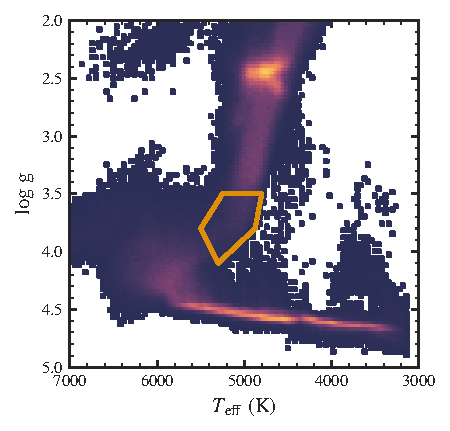
\includegraphics{logg_jack.pdf}
    \caption[Subgiant Selection]{
        A Kiel diagram of \apogee{} stars. Following \citetjack, I select \gls{subgiant}s in the orange polygon (see Equation \ref{eq:subgiant_selection}). These stars have not yet experienced first dredge-up, so their photospheric C and N abundances should reflect their birth mixture.
    }
    \label{fig:subgiant_selection}
\end{figure}












\newpage
\chapter{Low-Mass Stellar Evolution}\label{sec:stel_evo}
For reference, I include here a brief summary of the physics behind carbon production in \glspl{lowmass}.
\Glspl{lowmass} ($\lesssim 8 M_\odot$, like our sun), are born when they are fusing H into He. Typically, the dominant process is through the aptly named \textit{pp chain}, which takes four protons $\proton$ and releases a He nucleus $\alpha$, positrons $\beta^{+}$, photons $\gamma$, and electron neutrinos $\nu_{\rm e}$.
\begin{subequations}
    \begin{align}
        \proton + \proton &\longrightarrow \isotope[2][1]{H} + \beta^+ + \nu_{\rm e} \\
        \proton + \isotope[2][1]{H} &\longrightarrow \isotope[3][2]{He} + \gamma\\
        \proton + \isotope[3][2]{He} &\longrightarrow \isotope[4][2]{He} + \beta^+ + \nu_{\rm e}.
    \end{align}
\end{subequations}
However, when the core temperature becomes high enough, the \gls{cno} begins to activate. Starting with \isotope[12]{C}, the \gls{cno} is a series of proton captures that result in the creation of a new He nucleus.
\begin{subequations}\label{eq:cno_cycle}
\begin{align}
    \proton + \isotope[12]{C} &\longrightarrow \isotope[13]{N} + \gamma \\
    \isotope[13]{N} &\longrightarrow  \isotope[13]{C} + \beta^+ + \nu_{\rm e}  \\
    \proton + \isotope[13]{C}  &\longrightarrow \isotope[14]{N} + \gamma\\
    \proton + \isotope[14]{N}  &\longrightarrow \isotope[15]{O} + \gamma \label{eq:n14}\\
    \isotope[15]{O} &\longrightarrow  \isotope[15]{N} + \beta^{+} + \nu_{\rm e} \\
    \proton + \isotope[15]{N} &\longrightarrow \isotope[12]{C} + \alpha
\end{align}
\end{subequations}
(There are other less important minor branches of the \gls{cno} cycle
 \citep{solar-fusion}.)
The \gls{cno} is more intense at high metallicities, as the abundance of \isotope[12]{C} is higher. Since the slowest reaction in the \gls{cno} is the \isotope[14]{N} proton capture (Eq.~\ref{eq:n14}; also see \citealt{solar-fusion}), the net effect is to convert \isotope[12]{C} into \isotope[14]{N}. 

After the end of the main sequence (core H burning), a star begins to ascend the \gls{rgb}. The star first becomes a \gls{subgiant}, slightly more luminous and redder than the main sequence. Then, \gls{fdu} occurs when the contracting core drives convection currents through, bringing processed material from the core to the surface. Because of the \gls{cno}, the surface abundances of C will be lowered and N enhanced.

Stars with masses $\gtrsim 0.6M_\odot$ build up a large He core during the \gls{rgb}. Eventually, conditions are dense and hot enough for He to being to fuse, and the star now enters the He-burning phase. (Second dredge-up occurs during this transition.) As the next (accessible) stable isotope after He is C, the primary process to fuse He is through the triple-$\alpha$ process, where three He nuclei are combined to form \isotope[12]{C}.
\begin{subequations} \label{eq:triple_alpha}
\begin{align}
    \alpha + \alpha &\longrightarrow \isotope[8][4]{Be} \\ 
    \alpha + \isotope[8][4]{Be} &\longrightarrow \isotope[12][6]{C} + 2\gamma \\ 
\end{align}
Additionally, some \isotope[12][6]{C} may furthermore fuse into O, $\alpha + \isotope[12][6]{C} \longrightarrow \isotope[16][8]{O} + \gamma$.

When the star's core becomes full of C and O, the star finally enters the asymptotic giant branch phase (\agb). (Only the most massive low-mass stars burn further than O, creating some Mg, but these stars are a small fraction of low-mass stars.) An \agb\ star has a more complex structure, with an inert core, a He-burning shell, and an outer H-burning shell. The double shell structure causes instabilities towards the end of the \agb\ phase. In this thermally pupating phase, each pulse begins with a He-flash (where the He-shell becomes much more luminous). This flash causes the star to expand, driving convective currents that dredge up material from the CO core (\gls{tdu}), and fusion stops temporarily. The star settles again and stays stable for several Myr until the cycle repeats. During each He-flash, some material from the stellar surface is lost. This mass-loss is the source of \agb\ enrichment. Finally, the star losses enough mass such that the thermal pulses stop. The star becomes a white dwarf, left to cool for eternity.


\end{subequations}

\newpage
\chapter{Oxygen and Magnesium}\label{sec:alt_agb}

As I focus on constraining relative yields, I neglect O and Mg yield variations in the main text (excluding the uniform scaling of yields and \gls{massloading} in Section~\ref{sec:outflows}). There is substantial variation in predicted Mg yields (see Fig.~\ref{fig:y_mg}). Most models predict relatively flat trends metallicity (even with rotation as in \citealt{LC18}). However, the variation is significant and my adopted $\Yoc$ yield is much higher than most models. This is a known problem (see \citealt{emily+21}). \Gls{cc} models underpredict $[{\rm Mg}/{\rm O}]$, and the reason why is unknown. My results are independent of the choice of \cc\ element as I assume $[{\rm Mg}/{\rm O}]=0$.



\begin{figure}[htp]
    \centering
    \includegraphics{y_o_mg.pdf}
    \caption[O/Mg Yields]{Similar to the top panel of Fig.~\ref{fig:y_cc}, but for Mg.
    }
    \label{fig:y_mg}
\end{figure}



\chapter{Software}
Software that has contributed to this work:

\begin{itemize}
    \item \citet{OhioSupercomputerCenter1987}
    \item \VICE~\citep{JW20, james+21}
    \item \texttt{matplotlib} \citep{matplotlib}
    \item \texttt{scipy} \citep{scipy}
    \item \texttt{IPython} \citep{ipy}
    \item \texttt{pandas} \citep{pandas}
    \item \texttt{numpy} \citep{numpy}
    \item \texttt{astropy} \citep{astropy:2013, astropy:2018, astropy:2022}
    \item \texttt{seaborn} \citep{seaborn}
\end{itemize}


\chapter{Low-Mass Stellar Yield Models} \label{sec:oob_models}
    \cxi\ is from \citet{cristallo+11,cristallo+15}, \vxiii{} from \cite{ventura+13,ventura+14,ventura+18,vincenzo+21}, \kx{} from \citet{karakas10}, and \kxvi{} from \cite{KL16,karakas+18}
\renewcommand*{\arraystretch}{1.8}
\begin{table}[h]
    \centering
    \begin{tabular}{l p{2.2in} p{2.2in}}
    \toprule
    model & Masses/$M_\odot$ & $Z$ \\
    \midrule
    \hypertarget{C11}{\texttt{C11}} &
    1.3, 1.5, 2.0, 2.5, 3.0, 4.0, 5.0, 6.0
    & 0.0001, 0.0003, 0.001, 0.002, 0.003, 0.006, 0.008, 0.01, 0.014, 0.02 \\

    \hypertarget{K10}{\texttt{K10}} &
    1.0, 1.25, 1.5, 1.75, 1.9, 2.25, 2.5, 3.0, 3.5, 4.0, 4.5, 5.0, 5.5, 6.0 
    &  0.0001, 0.004, 0.008, 0.02. \\
    
    \hypertarget{V13}{\texttt{V13}} 
    & 1.5, 2.0, 2.5, 3.0, 3.5, 4.0, 4.5, 5.0, 6.0, 6.5, 7.0
    & 0.0003, 0.001, 0.002, 0.004, 0.008, 0.014, 0.04 \\
    
    \hypertarget{K16}{\texttt{K16}} 
     & 1.0, 1.25, 1.5, 1.75, 2.25, 2.5, 2.75, 3.0, 3.25, 3.5, 3.75, 4.0, 4.5, 5.0, 5.5, 6.0, 7.0
     & 0.0003, 0.001, 0.002, 0.004, 0.008, 0.014, 0.04 \\
         \bottomrule
    \end{tabular}
\end{table}
    

\chapter{Symbols}


\setlength{\tabcolsep}{0pt}
\begin{longtable}{p{0.2\textwidth} p{0.8\textwidth}}
    $[A/B]$ & 
    The abundance ratio between elements $A$ and $B$. $[A/B] =
    \log_{10}\left(A/B\right) - \log_{10}\left(A_{\sun}/B_{\sun}\right)$, i.e.
    $[A/B]$ is the logarithm of the ratio between A and B, scales such that
    $[A/B]=0$ for the sun. Solar abundances are as measured in
    \citet{asplund+09}. \\
    
$\alpha_{\rm AGB}$ & 
The multiplicative increase in \agb\ C production. See Eq.~\ref{eq:alpha}. \\


$\alpha_{\rm CC}$ &
The multiplicative increase in \cc\ C production. See Eq.~\ref{eq:alpha}. \\

$\eta$ & 
The mass outflow loading factor. $\eta$ is the ratio between ejected gas from the galaxy and star formation, i.e. $\eta = \dot{M}_{\rm outflow}/\dot{M}_\star$. \\

$\zeta$ & 
{The high-mass star carbon yield metallicity dependence. See Eq.~\ref{eq:zeta}}. \\

$\ensuremath{\dot{\Sigma}}$ & 
The surface mass density of star formation. \\

$M$ &
The mass of a star, in units of $M_\odot$ \\

$\ensuremath{M_\odot}$ &
The mass of the sun. $M_\odot = 1.989\times10^{33}$\,g.  \\


$\dot{M}_\star$ & 
The rate of star formation (mass of new stars per time interval). \\

$\dot{M}_{\rm X}$ &
The rate of change of the mass of element $X$. \\

$f_{\rm AGB}$ &
The fractional contribution of \agb\ stars to the total \gls{imfave} carbon yield at solar metallicity. See Eq.~\ref{eq:f_agb} \\ 

$R$ &
The galactocentric radius (distance from the galactic center) in kpc. \\ 

$\tilde{y}_{\rm C}^{\rm AGB}$ &
The per-star yield of C from \glspl{lowmass} of a given mass. In other words, the amount of new C an \agb\ star ejects divided by the initial mass of the star. \\ 

$y_{\rm C}^{\rm AGB}$ &
The \gls{imfave} yield of C from \glspl{lowmass}. \\ 

$y_{\rm C}^{\rm CC}$ &
The \gls{imfave} yield of C from \glspl{highmass}. \\ 

$y_{\rm Mg}^{\rm CC}$ &
The \gls{imfave} yield of Mg. \\ 

$Z_\odot$ &
The metallicity for the sun. $Z_\odot=0.014$.  \\ 

$Z$ &
The metallicity fraction, i.e. the mass fraction of all elements which are not H or He.  \\ 

$Z_X$ &
The mass fraction of element $X$. \\

\end{longtable}

\setlength{\tabcolsep}{6pt}
\renewcommand*{\arraystretch}{1}



\printglossary[type=\acronymtype,nonumberlist]


\printglossary




\end{document}




